\documentclass{article}
\usepackage{microtype}
\usepackage{graphicx}
\usepackage{booktabs}
\usepackage{hyperref}
\usepackage{icml2026}
\usepackage{amsmath,amssymb,amsthm}
\usepackage[capitalize,noabbrev]{cleveref}
\usepackage{enumitem}
\usepackage{tcolorbox}
\hypersetup{colorlinks=true,linkcolor=[RGB]{24,64,140},citecolor=[RGB]{24,64,140},urlcolor=[RGB]{24,64,140}}
\graphicspath{{figures/}}

\theoremstyle{plain}
\newtheorem{proposition}{Proposition}
\newtheorem{lemma}{Lemma}
\theoremstyle{remark}
\newtheorem{remark}{Remark}
\theoremstyle{definition}
\newtheorem{observation}{Observation}

% generated by analysis/icml_numbers.py; do not edit
\providecommand{\pending}[1]{\textbf{[PENDING: #1]}}
\newcommand{\GapAnchPerHeadGemmaBfcl}{+0.032}
\newcommand{\GapAnchPerHeadGemmaGlaive}{--}
\newcommand{\GapAnchPerHeadHiGemmaBfcl}{+0.06}
\newcommand{\GapAnchPerHeadHiGemmaGlaive}{--}
\newcommand{\GapAnchPerHeadHiLlamaOneBBfcl}{+0.04}
\newcommand{\GapAnchPerHeadHiLlamaOneBGlaive}{--}
\newcommand{\GapAnchPerHeadHiLlamaOneBLive}{--}
\newcommand{\GapAnchPerHeadHiLlamaThreeBBfcl}{--}
\newcommand{\GapAnchPerHeadHiLlamaThreeBGlaive}{--}
\newcommand{\GapAnchPerHeadHiMiniCpmBfcl}{+0.14}
\newcommand{\GapAnchPerHeadHiMiniCpmGlaive}{+0.34}
\newcommand{\GapAnchPerHeadHiMiniCpmLive}{+0.11}
\newcommand{\GapAnchPerHeadHiQwenThreeBfcl}{--}
\newcommand{\GapAnchPerHeadHiQwenThreeFiveBfcl}{+0.17}
\newcommand{\GapAnchPerHeadHiQwenThreeGlaive}{+0.14}
\newcommand{\GapAnchPerHeadLlamaOneBBfcl}{-0.005}
\newcommand{\GapAnchPerHeadLlamaOneBGlaive}{--}
\newcommand{\GapAnchPerHeadLlamaOneBLive}{--}
\newcommand{\GapAnchPerHeadLlamaThreeBBfcl}{--}
\newcommand{\GapAnchPerHeadLlamaThreeBGlaive}{--}
\newcommand{\GapAnchPerHeadLoGemmaBfcl}{+0.00}
\newcommand{\GapAnchPerHeadLoGemmaGlaive}{--}
\newcommand{\GapAnchPerHeadLoLlamaOneBBfcl}{-0.05}
\newcommand{\GapAnchPerHeadLoLlamaOneBGlaive}{--}
\newcommand{\GapAnchPerHeadLoLlamaOneBLive}{--}
\newcommand{\GapAnchPerHeadLoLlamaThreeBBfcl}{--}
\newcommand{\GapAnchPerHeadLoLlamaThreeBGlaive}{--}
\newcommand{\GapAnchPerHeadLoMiniCpmBfcl}{-0.02}
\newcommand{\GapAnchPerHeadLoMiniCpmGlaive}{-0.19}
\newcommand{\GapAnchPerHeadLoMiniCpmLive}{-0.08}
\newcommand{\GapAnchPerHeadLoQwenThreeBfcl}{--}
\newcommand{\GapAnchPerHeadLoQwenThreeFiveBfcl}{-0.03}
\newcommand{\GapAnchPerHeadLoQwenThreeGlaive}{-0.49}
\newcommand{\GapAnchPerHeadMiniCpmBfcl}{+0.053}
\newcommand{\GapAnchPerHeadMiniCpmGlaive}{+0.060}
\newcommand{\GapAnchPerHeadMiniCpmLive}{+0.010}
\newcommand{\GapAnchPerHeadQwenThreeBfcl}{--}
\newcommand{\GapAnchPerHeadQwenThreeFiveBfcl}{+0.079}
\newcommand{\GapAnchPerHeadQwenThreeGlaive}{-0.108}
\newcommand{\GapFloorGemmaBfcl}{+0.083}
\newcommand{\GapFloorGemmaGlaive}{+0.179}
\newcommand{\GapFloorHiGemmaBfcl}{+0.12}
\newcommand{\GapFloorHiGemmaGlaive}{+0.38}
\newcommand{\GapFloorHiLlamaOneBBfcl}{+0.27}
\newcommand{\GapFloorHiLlamaOneBGlaive}{+0.66}
\newcommand{\GapFloorHiLlamaOneBLive}{+0.17}
\newcommand{\GapFloorHiLlamaThreeBBfcl}{+0.33}
\newcommand{\GapFloorHiLlamaThreeBGlaive}{+0.60}
\newcommand{\GapFloorHiMiniCpmBfcl}{+0.35}
\newcommand{\GapFloorHiMiniCpmGlaive}{+0.43}
\newcommand{\GapFloorHiMiniCpmLive}{+0.31}
\newcommand{\GapFloorHiQwenThreeBfcl}{+0.27}
\newcommand{\GapFloorHiQwenThreeFiveBfcl}{+0.21}
\newcommand{\GapFloorHiQwenThreeGlaive}{+0.44}
\newcommand{\GapFloorLlamaOneBBfcl}{+0.210}
\newcommand{\GapFloorLlamaOneBGlaive}{+0.417}
\newcommand{\GapFloorLlamaOneBLive}{+0.074}
\newcommand{\GapFloorLlamaThreeBBfcl}{+0.262}
\newcommand{\GapFloorLlamaThreeBGlaive}{+0.406}
\newcommand{\GapFloorLoGemmaBfcl}{+0.05}
\newcommand{\GapFloorLoGemmaGlaive}{-0.09}
\newcommand{\GapFloorLoLlamaOneBBfcl}{+0.15}
\newcommand{\GapFloorLoLlamaOneBGlaive}{+0.06}
\newcommand{\GapFloorLoLlamaOneBLive}{-0.01}
\newcommand{\GapFloorLoLlamaThreeBBfcl}{+0.20}
\newcommand{\GapFloorLoLlamaThreeBGlaive}{+0.15}
\newcommand{\GapFloorLoMiniCpmBfcl}{+0.11}
\newcommand{\GapFloorLoMiniCpmGlaive}{-0.40}
\newcommand{\GapFloorLoMiniCpmLive}{+0.10}
\newcommand{\GapFloorLoQwenThreeBfcl}{+0.07}
\newcommand{\GapFloorLoQwenThreeFiveBfcl}{-0.00}
\newcommand{\GapFloorLoQwenThreeGlaive}{-0.45}
\newcommand{\GapFloorMiniCpmBfcl}{+0.244}
\newcommand{\GapFloorMiniCpmGlaive}{+0.025}
\newcommand{\GapFloorMiniCpmLive}{+0.204}
\newcommand{\GapFloorQwenThreeBfcl}{+0.175}
\newcommand{\GapFloorQwenThreeFiveBfcl}{+0.098}
\newcommand{\GapFloorQwenThreeGlaive}{-0.001}
\newcommand{\GapGemmaBfcl}{+0.242}
\newcommand{\GapGemmaGlaive}{+0.233}
\newcommand{\GapHiGemmaBfcl}{+0.30}
\newcommand{\GapHiGemmaGlaive}{+0.34}
\newcommand{\GapHiLlamaOneBBfcl}{+0.27}
\newcommand{\GapHiLlamaOneBGlaive}{+0.59}
\newcommand{\GapHiLlamaOneBLive}{+0.24}
\newcommand{\GapHiLlamaThreeBBfcl}{+0.23}
\newcommand{\GapHiLlamaThreeBGlaive}{+0.29}
\newcommand{\GapHiMiniCpmBfcl}{+0.09}
\newcommand{\GapHiMiniCpmGlaive}{+0.01}
\newcommand{\GapHiMiniCpmLive}{+0.02}
\newcommand{\GapHiQwenThreeBfcl}{+0.15}
\newcommand{\GapHiQwenThreeFiveBfcl}{-0.02}
\newcommand{\GapHiQwenThreeGlaive}{+0.21}
\newcommand{\GapLapEigFloorGemmaBfcl}{+0.032}
\newcommand{\GapLapEigFloorGemmaGlaive}{+0.133}
\newcommand{\GapLapEigFloorHiGemmaBfcl}{+0.07}
\newcommand{\GapLapEigFloorHiGemmaGlaive}{+0.36}
\newcommand{\GapLapEigFloorHiLlamaOneBBfcl}{+0.23}
\newcommand{\GapLapEigFloorHiLlamaOneBGlaive}{+0.64}
\newcommand{\GapLapEigFloorHiLlamaOneBLive}{+0.14}
\newcommand{\GapLapEigFloorHiLlamaThreeBBfcl}{+0.26}
\newcommand{\GapLapEigFloorHiLlamaThreeBGlaive}{+0.57}
\newcommand{\GapLapEigFloorHiMiniCpmBfcl}{+0.29}
\newcommand{\GapLapEigFloorHiMiniCpmGlaive}{+0.41}
\newcommand{\GapLapEigFloorHiMiniCpmLive}{+0.25}
\newcommand{\GapLapEigFloorHiQwenThreeBfcl}{+0.21}
\newcommand{\GapLapEigFloorHiQwenThreeFiveBfcl}{+0.12}
\newcommand{\GapLapEigFloorHiQwenThreeGlaive}{+0.38}
\newcommand{\GapLapEigFloorLlamaOneBBfcl}{+0.163}
\newcommand{\GapLapEigFloorLlamaOneBGlaive}{+0.396}
\newcommand{\GapLapEigFloorLlamaOneBLive}{+0.046}
\newcommand{\GapLapEigFloorLlamaThreeBBfcl}{+0.201}
\newcommand{\GapLapEigFloorLlamaThreeBGlaive}{+0.335}
\newcommand{\GapLapEigFloorLoGemmaBfcl}{-0.00}
\newcommand{\GapLapEigFloorLoGemmaGlaive}{-0.10}
\newcommand{\GapLapEigFloorLoLlamaOneBBfcl}{+0.10}
\newcommand{\GapLapEigFloorLoLlamaOneBGlaive}{+0.04}
\newcommand{\GapLapEigFloorLoLlamaOneBLive}{-0.05}
\newcommand{\GapLapEigFloorLoLlamaThreeBBfcl}{+0.14}
\newcommand{\GapLapEigFloorLoLlamaThreeBGlaive}{+0.05}
\newcommand{\GapLapEigFloorLoMiniCpmBfcl}{+0.09}
\newcommand{\GapLapEigFloorLoMiniCpmGlaive}{-0.45}
\newcommand{\GapLapEigFloorLoMiniCpmLive}{+0.01}
\newcommand{\GapLapEigFloorLoQwenThreeBfcl}{+0.00}
\newcommand{\GapLapEigFloorLoQwenThreeFiveBfcl}{-0.09}
\newcommand{\GapLapEigFloorLoQwenThreeGlaive}{-0.32}
\newcommand{\GapLapEigFloorMiniCpmBfcl}{+0.194}
\newcommand{\GapLapEigFloorMiniCpmGlaive}{-0.033}
\newcommand{\GapLapEigFloorMiniCpmLive}{+0.130}
\newcommand{\GapLapEigFloorQwenThreeBfcl}{+0.110}
\newcommand{\GapLapEigFloorQwenThreeFiveBfcl}{+0.017}
\newcommand{\GapLapEigFloorQwenThreeGlaive}{+0.001}
\newcommand{\GapLlamaOneBBfcl}{+0.200}
\newcommand{\GapLlamaOneBGlaive}{+0.379}
\newcommand{\GapLlamaOneBLive}{+0.119}
\newcommand{\GapLlamaThreeBBfcl}{+0.172}
\newcommand{\GapLlamaThreeBGlaive}{+0.163}
\newcommand{\GapLoGemmaBfcl}{+0.19}
\newcommand{\GapLoGemmaGlaive}{+0.11}
\newcommand{\GapLoLlamaOneBBfcl}{+0.12}
\newcommand{\GapLoLlamaOneBGlaive}{+0.15}
\newcommand{\GapLoLlamaOneBLive}{-0.00}
\newcommand{\GapLoLlamaThreeBBfcl}{+0.11}
\newcommand{\GapLoLlamaThreeBGlaive}{+0.05}
\newcommand{\GapLoMiniCpmBfcl}{-0.13}
\newcommand{\GapLoMiniCpmGlaive}{-0.51}
\newcommand{\GapLoMiniCpmLive}{-0.16}
\newcommand{\GapLoQwenThreeBfcl}{-0.06}
\newcommand{\GapLoQwenThreeFiveBfcl}{-0.18}
\newcommand{\GapLoQwenThreeGlaive}{-0.65}
\newcommand{\GapMiniCpmBfcl}{-0.008}
\newcommand{\GapMiniCpmGlaive}{-0.203}
\newcommand{\GapMiniCpmLive}{-0.051}
\newcommand{\GapPerHeadAvgGemmaBfcl}{+0.019}
\newcommand{\GapPerHeadAvgGemmaGlaive}{+0.099}
\newcommand{\GapPerHeadAvgHiGemmaBfcl}{+0.05}
\newcommand{\GapPerHeadAvgHiGemmaGlaive}{+0.23}
\newcommand{\GapPerHeadAvgHiLlamaOneBBfcl}{+0.20}
\newcommand{\GapPerHeadAvgHiLlamaOneBGlaive}{+0.55}
\newcommand{\GapPerHeadAvgHiLlamaOneBLive}{+0.25}
\newcommand{\GapPerHeadAvgHiLlamaThreeBBfcl}{+0.27}
\newcommand{\GapPerHeadAvgHiLlamaThreeBGlaive}{+0.44}
\newcommand{\GapPerHeadAvgHiMiniCpmBfcl}{+0.16}
\newcommand{\GapPerHeadAvgHiMiniCpmGlaive}{+0.42}
\newcommand{\GapPerHeadAvgHiMiniCpmLive}{+0.18}
\newcommand{\GapPerHeadAvgHiQwenThreeBfcl}{+0.24}
\newcommand{\GapPerHeadAvgHiQwenThreeFiveBfcl}{+0.17}
\newcommand{\GapPerHeadAvgHiQwenThreeGlaive}{+0.63}
\newcommand{\GapPerHeadAvgLlamaOneBBfcl}{+0.137}
\newcommand{\GapPerHeadAvgLlamaOneBGlaive}{+0.344}
\newcommand{\GapPerHeadAvgLlamaOneBLive}{+0.152}
\newcommand{\GapPerHeadAvgLlamaThreeBBfcl}{+0.204}
\newcommand{\GapPerHeadAvgLlamaThreeBGlaive}{+0.278}
\newcommand{\GapPerHeadAvgLoGemmaBfcl}{-0.01}
\newcommand{\GapPerHeadAvgLoGemmaGlaive}{-0.01}
\newcommand{\GapPerHeadAvgLoLlamaOneBBfcl}{+0.08}
\newcommand{\GapPerHeadAvgLoLlamaOneBGlaive}{+0.11}
\newcommand{\GapPerHeadAvgLoLlamaOneBLive}{+0.05}
\newcommand{\GapPerHeadAvgLoLlamaThreeBBfcl}{+0.14}
\newcommand{\GapPerHeadAvgLoLlamaThreeBGlaive}{+0.07}
\newcommand{\GapPerHeadAvgLoMiniCpmBfcl}{-0.03}
\newcommand{\GapPerHeadAvgLoMiniCpmGlaive}{-0.27}
\newcommand{\GapPerHeadAvgLoMiniCpmLive}{-0.05}
\newcommand{\GapPerHeadAvgLoQwenThreeBfcl}{-0.06}
\newcommand{\GapPerHeadAvgLoQwenThreeFiveBfcl}{-0.10}
\newcommand{\GapPerHeadAvgLoQwenThreeGlaive}{-0.01}
\newcommand{\GapPerHeadAvgMiniCpmBfcl}{+0.066}
\newcommand{\GapPerHeadAvgMiniCpmGlaive}{+0.077}
\newcommand{\GapPerHeadAvgMiniCpmLive}{+0.067}
\newcommand{\GapPerHeadAvgQwenThreeBfcl}{+0.104}
\newcommand{\GapPerHeadAvgQwenThreeFiveBfcl}{+0.032}
\newcommand{\GapPerHeadAvgQwenThreeGlaive}{+0.336}
\newcommand{\GapPerHeadLapEigGemmaBfcl}{+0.005}
\newcommand{\GapPerHeadLapEigGemmaGlaive}{-0.003}
\newcommand{\GapPerHeadLapEigHiGemmaBfcl}{+0.04}
\newcommand{\GapPerHeadLapEigHiGemmaGlaive}{+0.16}
\newcommand{\GapPerHeadLapEigHiLlamaOneBBfcl}{+0.04}
\newcommand{\GapPerHeadLapEigHiLlamaOneBGlaive}{+0.08}
\newcommand{\GapPerHeadLapEigHiLlamaOneBLive}{+0.15}
\newcommand{\GapPerHeadLapEigHiLlamaThreeBBfcl}{+0.06}
\newcommand{\GapPerHeadLapEigHiLlamaThreeBGlaive}{+0.15}
\newcommand{\GapPerHeadLapEigHiMiniCpmBfcl}{+0.08}
\newcommand{\GapPerHeadLapEigHiMiniCpmGlaive}{+0.41}
\newcommand{\GapPerHeadLapEigHiMiniCpmLive}{+0.12}
\newcommand{\GapPerHeadLapEigHiQwenThreeBfcl}{+0.13}
\newcommand{\GapPerHeadLapEigHiQwenThreeFiveBfcl}{+0.15}
\newcommand{\GapPerHeadLapEigHiQwenThreeGlaive}{+0.35}
\newcommand{\GapPerHeadLapEigLlamaOneBBfcl}{-0.003}
\newcommand{\GapPerHeadLapEigLlamaOneBGlaive}{+0.011}
\newcommand{\GapPerHeadLapEigLlamaOneBLive}{+0.042}
\newcommand{\GapPerHeadLapEigLlamaThreeBBfcl}{+0.011}
\newcommand{\GapPerHeadLapEigLlamaThreeBGlaive}{+0.021}
\newcommand{\GapPerHeadLapEigLoGemmaBfcl}{-0.03}
\newcommand{\GapPerHeadLapEigLoGemmaGlaive}{-0.11}
\newcommand{\GapPerHeadLapEigLoLlamaOneBBfcl}{-0.05}
\newcommand{\GapPerHeadLapEigLoLlamaOneBGlaive}{-0.09}
\newcommand{\GapPerHeadLapEigLoLlamaOneBLive}{-0.05}
\newcommand{\GapPerHeadLapEigLoLlamaThreeBBfcl}{-0.03}
\newcommand{\GapPerHeadLapEigLoLlamaThreeBGlaive}{-0.13}
\newcommand{\GapPerHeadLapEigLoMiniCpmBfcl}{-0.10}
\newcommand{\GapPerHeadLapEigLoMiniCpmGlaive}{-0.31}
\newcommand{\GapPerHeadLapEigLoMiniCpmLive}{-0.11}
\newcommand{\GapPerHeadLapEigLoQwenThreeBfcl}{-0.10}
\newcommand{\GapPerHeadLapEigLoQwenThreeFiveBfcl}{-0.07}
\newcommand{\GapPerHeadLapEigLoQwenThreeGlaive}{-0.14}
\newcommand{\GapPerHeadLapEigMiniCpmBfcl}{-0.021}
\newcommand{\GapPerHeadLapEigMiniCpmGlaive}{+0.061}
\newcommand{\GapPerHeadLapEigMiniCpmLive}{+0.016}
\newcommand{\GapPerHeadLapEigQwenThreeBfcl}{+0.019}
\newcommand{\GapPerHeadLapEigQwenThreeFiveBfcl}{+0.040}
\newcommand{\GapPerHeadLapEigQwenThreeGlaive}{+0.103}
\newcommand{\GapProbePerHeadGemmaBfcl}{+0.045}
\newcommand{\GapProbePerHeadGemmaGlaive}{+0.049}
\newcommand{\GapProbePerHeadHiGemmaBfcl}{+0.08}
\newcommand{\GapProbePerHeadHiGemmaGlaive}{+0.18}
\newcommand{\GapProbePerHeadHiLlamaOneBBfcl}{+0.09}
\newcommand{\GapProbePerHeadHiLlamaOneBGlaive}{+0.05}
\newcommand{\GapProbePerHeadHiLlamaOneBLive}{+0.06}
\newcommand{\GapProbePerHeadHiLlamaThreeBBfcl}{+0.10}
\newcommand{\GapProbePerHeadHiLlamaThreeBGlaive}{+0.18}
\newcommand{\GapProbePerHeadHiMiniCpmBfcl}{+0.16}
\newcommand{\GapProbePerHeadHiMiniCpmGlaive}{+0.34}
\newcommand{\GapProbePerHeadHiMiniCpmLive}{+0.16}
\newcommand{\GapProbePerHeadHiQwenThreeBfcl}{+0.16}
\newcommand{\GapProbePerHeadHiQwenThreeFiveBfcl}{+0.15}
\newcommand{\GapProbePerHeadHiQwenThreeGlaive}{+0.22}
\newcommand{\GapProbePerHeadLlamaOneBBfcl}{+0.050}
\newcommand{\GapProbePerHeadLlamaOneBGlaive}{+0.011}
\newcommand{\GapProbePerHeadLlamaOneBLive}{-0.014}
\newcommand{\GapProbePerHeadLlamaThreeBBfcl}{+0.051}
\newcommand{\GapProbePerHeadLlamaThreeBGlaive}{+0.050}
\newcommand{\GapProbePerHeadLoGemmaBfcl}{+0.00}
\newcommand{\GapProbePerHeadLoGemmaGlaive}{-0.14}
\newcommand{\GapProbePerHeadLoLlamaOneBBfcl}{+0.01}
\newcommand{\GapProbePerHeadLoLlamaOneBGlaive}{-0.03}
\newcommand{\GapProbePerHeadLoLlamaOneBLive}{-0.11}
\newcommand{\GapProbePerHeadLoLlamaThreeBBfcl}{+0.01}
\newcommand{\GapProbePerHeadLoLlamaThreeBGlaive}{-0.02}
\newcommand{\GapProbePerHeadLoMiniCpmBfcl}{-0.05}
\newcommand{\GapProbePerHeadLoMiniCpmGlaive}{-0.35}
\newcommand{\GapProbePerHeadLoMiniCpmLive}{-0.07}
\newcommand{\GapProbePerHeadLoQwenThreeBfcl}{-0.04}
\newcommand{\GapProbePerHeadLoQwenThreeFiveBfcl}{-0.06}
\newcommand{\GapProbePerHeadLoQwenThreeGlaive}{-0.59}
\newcommand{\GapProbePerHeadMiniCpmBfcl}{+0.071}
\newcommand{\GapProbePerHeadMiniCpmGlaive}{-0.003}
\newcommand{\GapProbePerHeadMiniCpmLive}{+0.058}
\newcommand{\GapProbePerHeadQwenThreeBfcl}{+0.046}
\newcommand{\GapProbePerHeadQwenThreeFiveBfcl}{+0.042}
\newcommand{\GapProbePerHeadQwenThreeGlaive}{-0.106}
\newcommand{\GapQwenThreeBfcl}{+0.051}
\newcommand{\GapQwenThreeFiveBfcl}{-0.099}
\newcommand{\GapQwenThreeGlaive}{-0.191}
\newcommand{\aucAnchGemmaBfcl}{0.935}
\newcommand{\aucAnchGemmaGlaive}{--}
\newcommand{\aucAnchLlamaOneBBfcl}{0.806}
\newcommand{\aucAnchLlamaOneBGlaive}{--}
\newcommand{\aucAnchLlamaOneBLive}{--}
\newcommand{\aucAnchLlamaThreeBBfcl}{--}
\newcommand{\aucAnchLlamaThreeBGlaive}{--}
\newcommand{\aucAnchMiniCpmBfcl}{0.789}
\newcommand{\aucAnchMiniCpmGlaive}{0.773}
\newcommand{\aucAnchMiniCpmLive}{0.699}
\newcommand{\aucAnchQwenThreeBfcl}{--}
\newcommand{\aucAnchQwenThreeFiveBfcl}{0.728}
\newcommand{\aucAnchQwenThreeGlaive}{0.674}
\newcommand{\aucBestConfGemmaBfcl}{0.600}
\newcommand{\aucBestConfGemmaGlaive}{0.650}
\newcommand{\aucBestConfLlamaOneBBfcl}{0.680}
\newcommand{\aucBestConfLlamaOneBGlaive}{0.579}
\newcommand{\aucBestConfLlamaOneBLive}{0.661}
\newcommand{\aucBestConfLlamaThreeBBfcl}{0.712}
\newcommand{\aucBestConfLlamaThreeBGlaive}{0.773}
\newcommand{\aucBestConfMiniCpmBfcl}{0.819}
\newcommand{\aucBestConfMiniCpmGlaive}{0.749}
\newcommand{\aucBestConfMiniCpmLive}{0.795}
\newcommand{\aucBestConfQwenThreeBfcl}{0.741}
\newcommand{\aucBestConfQwenThreeFiveBfcl}{0.814}
\newcommand{\aucBestConfQwenThreeGlaive}{0.908}
\newcommand{\aucConfGemmaBfcl}{0.707}
\newcommand{\aucConfGemmaGlaive}{0.650}
\newcommand{\aucConfLlamaOneBBfcl}{0.661}
\newcommand{\aucConfLlamaOneBGlaive}{0.579}
\newcommand{\aucConfLlamaOneBLive}{0.661}
\newcommand{\aucConfLlamaThreeBBfcl}{0.712}
\newcommand{\aucConfLlamaThreeBGlaive}{0.773}
\newcommand{\aucConfMiniCpmBfcl}{0.815}
\newcommand{\aucConfMiniCpmGlaive}{0.913}
\newcommand{\aucConfMiniCpmLive}{0.798}
\newcommand{\aucConfQwenThreeBfcl}{0.741}
\newcommand{\aucConfQwenThreeFiveBfcl}{0.789}
\newcommand{\aucConfQwenThreeGlaive}{0.867}
\newcommand{\aucFloorGemmaBfcl}{0.866}
\newcommand{\aucFloorGemmaGlaive}{0.704}
\newcommand{\aucFloorLlamaOneBBfcl}{0.652}
\newcommand{\aucFloorLlamaOneBGlaive}{0.540}
\newcommand{\aucFloorLlamaOneBLive}{0.707}
\newcommand{\aucFloorLlamaThreeBBfcl}{0.621}
\newcommand{\aucFloorLlamaThreeBGlaive}{0.529}
\newcommand{\aucFloorMiniCpmBfcl}{0.564}
\newcommand{\aucFloorMiniCpmGlaive}{0.685}
\newcommand{\aucFloorMiniCpmLive}{0.543}
\newcommand{\aucFloorQwenThreeBfcl}{0.616}
\newcommand{\aucFloorQwenThreeFiveBfcl}{0.592}
\newcommand{\aucFloorQwenThreeGlaive}{0.677}
\newcommand{\aucGramGemmaBfcl}{0.879}
\newcommand{\aucGramGemmaGlaive}{0.719}
\newcommand{\aucGramLlamaOneBBfcl}{0.732}
\newcommand{\aucGramLlamaOneBGlaive}{0.697}
\newcommand{\aucGramLlamaOneBLive}{0.695}
\newcommand{\aucGramLlamaThreeBBfcl}{0.715}
\newcommand{\aucGramLlamaThreeBGlaive}{0.622}
\newcommand{\aucGramMiniCpmBfcl}{0.571}
\newcommand{\aucGramMiniCpmGlaive}{0.692}
\newcommand{\aucGramMiniCpmLive}{0.609}
\newcommand{\aucGramQwenThreeBfcl}{0.618}
\newcommand{\aucGramQwenThreeFiveBfcl}{0.637}
\newcommand{\aucGramQwenThreeGlaive}{0.813}
\newcommand{\aucHeadAvgGemmaBfcl}{0.884}
\newcommand{\aucHeadAvgGemmaGlaive}{0.736}
\newcommand{\aucHeadAvgLlamaOneBBfcl}{0.675}
\newcommand{\aucHeadAvgLlamaOneBGlaive}{0.602}
\newcommand{\aucHeadAvgLlamaOneBLive}{0.643}
\newcommand{\aucHeadAvgLlamaThreeBBfcl}{0.629}
\newcommand{\aucHeadAvgLlamaThreeBGlaive}{0.607}
\newcommand{\aucHeadAvgMiniCpmBfcl}{0.670}
\newcommand{\aucHeadAvgMiniCpmGlaive}{0.635}
\newcommand{\aucHeadAvgMiniCpmLive}{0.622}
\newcommand{\aucHeadAvgQwenThreeBfcl}{0.642}
\newcommand{\aucHeadAvgQwenThreeFiveBfcl}{0.617}
\newcommand{\aucHeadAvgQwenThreeGlaive}{0.445}
\newcommand{\aucLapEigGemmaBfcl}{0.898}
\newcommand{\aucLapEigGemmaGlaive}{0.837}
\newcommand{\aucLapEigLlamaOneBBfcl}{0.815}
\newcommand{\aucLapEigLlamaOneBGlaive}{0.936}
\newcommand{\aucLapEigLlamaOneBLive}{0.752}
\newcommand{\aucLapEigLlamaThreeBBfcl}{0.822}
\newcommand{\aucLapEigLlamaThreeBGlaive}{0.864}
\newcommand{\aucLapEigMiniCpmBfcl}{0.758}
\newcommand{\aucLapEigMiniCpmGlaive}{0.652}
\newcommand{\aucLapEigMiniCpmLive}{0.673}
\newcommand{\aucLapEigQwenThreeBfcl}{0.727}
\newcommand{\aucLapEigQwenThreeFiveBfcl}{0.609}
\newcommand{\aucLapEigQwenThreeGlaive}{0.678}
\newcommand{\aucLookbackGemmaBfcl}{0.928}
\newcommand{\aucLookbackGemmaGlaive}{0.786}
\newcommand{\aucLookbackLlamaOneBBfcl}{0.792}
\newcommand{\aucLookbackLlamaOneBGlaive}{0.940}
\newcommand{\aucLookbackLlamaOneBLive}{0.804}
\newcommand{\aucLookbackLlamaThreeBBfcl}{0.832}
\newcommand{\aucLookbackLlamaThreeBGlaive}{0.883}
\newcommand{\aucLookbackMiniCpmBfcl}{0.780}
\newcommand{\aucLookbackMiniCpmGlaive}{0.723}
\newcommand{\aucLookbackMiniCpmLive}{0.721}
\newcommand{\aucLookbackQwenThreeBfcl}{0.778}
\newcommand{\aucLookbackQwenThreeFiveBfcl}{0.664}
\newcommand{\aucLookbackQwenThreeGlaive}{0.709}
\newcommand{\aucPerHeadGemmaBfcl}{0.903}
\newcommand{\aucPerHeadGemmaGlaive}{0.834}
\newcommand{\aucPerHeadLlamaOneBBfcl}{0.812}
\newcommand{\aucPerHeadLlamaOneBGlaive}{0.947}
\newcommand{\aucPerHeadLlamaOneBLive}{0.795}
\newcommand{\aucPerHeadLlamaThreeBBfcl}{0.833}
\newcommand{\aucPerHeadLlamaThreeBGlaive}{0.885}
\newcommand{\aucPerHeadMiniCpmBfcl}{0.736}
\newcommand{\aucPerHeadMiniCpmGlaive}{0.713}
\newcommand{\aucPerHeadMiniCpmLive}{0.688}
\newcommand{\aucPerHeadQwenThreeBfcl}{0.745}
\newcommand{\aucPerHeadQwenThreeFiveBfcl}{0.649}
\newcommand{\aucPerHeadQwenThreeGlaive}{0.781}
\newcommand{\aucProbeGemmaBfcl}{0.949}
\newcommand{\aucProbeGemmaGlaive}{0.883}
\newcommand{\aucProbeLlamaOneBBfcl}{0.861}
\newcommand{\aucProbeLlamaOneBGlaive}{0.957}
\newcommand{\aucProbeLlamaOneBLive}{0.780}
\newcommand{\aucProbeLlamaThreeBBfcl}{0.884}
\newcommand{\aucProbeLlamaThreeBGlaive}{0.936}
\newcommand{\aucProbeMiniCpmBfcl}{0.808}
\newcommand{\aucProbeMiniCpmGlaive}{0.710}
\newcommand{\aucProbeMiniCpmLive}{0.747}
\newcommand{\aucProbeQwenThreeBfcl}{0.791}
\newcommand{\aucProbeQwenThreeFiveBfcl}{0.691}
\newcommand{\aucProbeQwenThreeGlaive}{0.676}
\newcommand{\aucResDynGemmaBfcl}{0.894}
\newcommand{\aucResDynGemmaGlaive}{0.796}
\newcommand{\aucResDynLlamaOneBBfcl}{0.735}
\newcommand{\aucResDynLlamaOneBGlaive}{0.644}
\newcommand{\aucResDynLlamaOneBLive}{0.680}
\newcommand{\aucResDynLlamaThreeBBfcl}{0.688}
\newcommand{\aucResDynLlamaThreeBGlaive}{0.764}
\newcommand{\aucResDynMiniCpmBfcl}{0.649}
\newcommand{\aucResDynMiniCpmGlaive}{0.606}
\newcommand{\aucResDynMiniCpmLive}{0.551}
\newcommand{\aucResDynQwenThreeBfcl}{0.632}
\newcommand{\aucResDynQwenThreeFiveBfcl}{0.626}
\newcommand{\aucResDynQwenThreeGlaive}{0.843}
\newcommand{\aucSinkGemmaBfcl}{0.929}
\newcommand{\aucSinkGemmaGlaive}{--}
\newcommand{\aucSinkLlamaOneBBfcl}{0.833}
\newcommand{\aucSinkLlamaOneBGlaive}{--}
\newcommand{\aucSinkLlamaOneBLive}{--}
\newcommand{\aucSinkLlamaThreeBBfcl}{--}
\newcommand{\aucSinkLlamaThreeBGlaive}{--}
\newcommand{\aucSinkMiniCpmBfcl}{0.799}
\newcommand{\aucSinkMiniCpmGlaive}{0.690}
\newcommand{\aucSinkMiniCpmLive}{0.705}
\newcommand{\aucSinkQwenThreeBfcl}{--}
\newcommand{\aucSinkQwenThreeFiveBfcl}{0.660}
\newcommand{\aucSinkQwenThreeGlaive}{0.702}
\newcommand{\aucTokenLevelGemmaBfcl}{0.946}
\newcommand{\aucTokenLevelGemmaGlaive}{0.898}
\newcommand{\aucTokenLevelLlamaOneBBfcl}{0.832}
\newcommand{\aucTokenLevelLlamaOneBGlaive}{0.971}
\newcommand{\aucTokenLevelLlamaOneBLive}{0.774}
\newcommand{\aucTokenLevelLlamaThreeBBfcl}{0.846}
\newcommand{\aucTokenLevelLlamaThreeBGlaive}{0.863}
\newcommand{\aucTokenLevelMiniCpmBfcl}{0.810}
\newcommand{\aucTokenLevelMiniCpmGlaive}{0.760}
\newcommand{\aucTokenLevelMiniCpmLive}{0.737}
\newcommand{\aucTokenLevelQwenThreeBfcl}{0.734}
\newcommand{\aucTokenLevelQwenThreeFiveBfcl}{0.719}
\newcommand{\aucTokenLevelQwenThreeGlaive}{0.790}
\newcommand{\bestConfShrinkMax}{0.019}
\newcommand{\bestConfShrinkMean}{-0.044}
\newcommand{\budgetFullPosLlamaOneB}{236}
\newcommand{\budgetFullPosLlamaThreeB}{157}
\newcommand{\budgetGapAtMinLlamaOneB}{+0.215}
\newcommand{\budgetGapAtMinLlamaThreeB}{+0.149}
\newcommand{\budgetGapFullLlamaOneB}{+0.244}
\newcommand{\budgetGapFullLlamaThreeB}{+0.182}
\newcommand{\budgetMinPosLlamaOneB}{51}
\newcommand{\budgetMinPosLlamaThreeB}{51}
\newcommand{\budgetProbeAtMinLlamaOneB}{0.853}
\newcommand{\budgetProbeAtMinLlamaThreeB}{0.861}
\newcommand{\budgetProbeDropLlamaOneB}{0.029}
\newcommand{\budgetProbeDropLlamaThreeB}{0.034}
\newcommand{\budgetProbeFullLlamaOneB}{0.882}
\newcommand{\budgetProbeFullLlamaThreeB}{0.894}
\newcommand{\ckptExactFloor}{0.100}
\newcommand{\ckptGapGemma}{+0.237}
\newcommand{\ckptGapLlamaOneB}{+0.233}
\newcommand{\ckptGapLlamaThreeB}{+0.167}
\newcommand{\ckptGapMiniCpm}{-0.030}
\newcommand{\ckptGapQwenThree}{+0.051}
\newcommand{\ckptGapQwenThreeFive}{-0.099}
\newcommand{\ckptSeparated}{yes}
\newcommand{\diffConfWithinLlamaOneB}{0.643}
\newcommand{\diffConfWithinLlamaThreeB}{0.700}
\newcommand{\diffConfWithinMiniCpm}{0.844}
\newcommand{\diffConfWithinQwenThree}{0.805}
\newcommand{\diffConfWithinQwenThreeFive}{0.806}
\newcommand{\diffGapRawLlamaOneB}{+0.247}
\newcommand{\diffGapRawLlamaThreeB}{+0.179}
\newcommand{\diffGapRawMiniCpm}{-0.048}
\newcommand{\diffGapRawQwenThree}{+0.009}
\newcommand{\diffGapRawQwenThreeFive}{-0.098}
\newcommand{\diffGapWithinLlamaOneB}{+0.250}
\newcommand{\diffGapWithinLlamaThreeB}{+0.192}
\newcommand{\diffGapWithinMiniCpm}{-0.107}
\newcommand{\diffGapWithinQwenThree}{-0.079}
\newcommand{\diffGapWithinQwenThreeFive}{-0.130}
\newcommand{\diffOnlyLlamaOneB}{0.670}
\newcommand{\diffOnlyLlamaThreeB}{0.715}
\newcommand{\diffOnlyMax}{0.813}
\newcommand{\diffOnlyMin}{0.670}
\newcommand{\diffOnlyMiniCpm}{0.771}
\newcommand{\diffOnlyQwenThree}{0.813}
\newcommand{\diffOnlyQwenThreeFive}{0.708}
\newcommand{\diffProbeWithinLlamaOneB}{0.893}
\newcommand{\diffProbeWithinLlamaThreeB}{0.892}
\newcommand{\diffProbeWithinMiniCpm}{0.736}
\newcommand{\diffProbeWithinQwenThree}{0.726}
\newcommand{\diffProbeWithinQwenThreeFive}{0.676}
\newcommand{\failGemmaBfcl}{84}
\newcommand{\failGemmaGlaive}{29}
\newcommand{\failLlamaOneBBfcl}{64}
\newcommand{\failLlamaOneBGlaive}{45}
\newcommand{\failLlamaOneBLive}{72}
\newcommand{\failLlamaThreeBBfcl}{37}
\newcommand{\failLlamaThreeBGlaive}{16}
\newcommand{\failMiniCpmBfcl}{11}
\newcommand{\failMiniCpmGlaive}{2}
\newcommand{\failMiniCpmLive}{21}
\newcommand{\failQwenThreeBfcl}{11}
\newcommand{\failQwenThreeFiveBfcl}{39}
\newcommand{\failQwenThreeGlaive}{4}
\newcommand{\gapBestConfidenceMax}{-0.011}
\newcommand{\gapBestGemmaBfcl}{+0.349}
\newcommand{\gapBestGemmaGlaive}{+0.233}
\newcommand{\gapBestHiGemmaBfcl}{+0.41}
\newcommand{\gapBestHiGemmaGlaive}{+0.33}
\newcommand{\gapBestHiLlamaOneBBfcl}{+0.25}
\newcommand{\gapBestHiLlamaOneBGlaive}{+0.58}
\newcommand{\gapBestHiLlamaOneBLive}{+0.23}
\newcommand{\gapBestHiLlamaThreeBBfcl}{+0.23}
\newcommand{\gapBestHiLlamaThreeBGlaive}{+0.28}
\newcommand{\gapBestHiMiniCpmBfcl}{+0.07}
\newcommand{\gapBestHiMiniCpmGlaive}{+0.27}
\newcommand{\gapBestHiMiniCpmLive}{+0.00}
\newcommand{\gapBestHiQwenThreeBfcl}{+0.15}
\newcommand{\gapBestHiQwenThreeFiveBfcl}{-0.05}
\newcommand{\gapBestHiQwenThreeGlaive}{+0.07}
\newcommand{\gapBestInternalsMin}{+0.181}
\newcommand{\gapBestLlamaOneBBfcl}{+0.181}
\newcommand{\gapBestLlamaOneBGlaive}{+0.379}
\newcommand{\gapBestLlamaOneBLive}{+0.119}
\newcommand{\gapBestLlamaThreeBBfcl}{+0.172}
\newcommand{\gapBestLlamaThreeBGlaive}{+0.163}
\newcommand{\gapBestLoGemmaBfcl}{+0.29}
\newcommand{\gapBestLoGemmaGlaive}{+0.12}
\newcommand{\gapBestLoLlamaOneBBfcl}{+0.11}
\newcommand{\gapBestLoLlamaOneBGlaive}{+0.19}
\newcommand{\gapBestLoLlamaOneBLive}{+0.01}
\newcommand{\gapBestLoLlamaThreeBBfcl}{+0.12}
\newcommand{\gapBestLoLlamaThreeBGlaive}{+0.07}
\newcommand{\gapBestLoMiniCpmBfcl}{-0.09}
\newcommand{\gapBestLoMiniCpmGlaive}{-0.31}
\newcommand{\gapBestLoMiniCpmLive}{-0.11}
\newcommand{\gapBestLoQwenThreeBfcl}{-0.05}
\newcommand{\gapBestLoQwenThreeFiveBfcl}{-0.20}
\newcommand{\gapBestLoQwenThreeGlaive}{-0.44}
\newcommand{\gapBestMiniCpmBfcl}{-0.011}
\newcommand{\gapBestMiniCpmGlaive}{-0.039}
\newcommand{\gapBestMiniCpmLive}{-0.049}
\newcommand{\gapBestQwenThreeBfcl}{+0.051}
\newcommand{\gapBestQwenThreeFiveBfcl}{-0.123}
\newcommand{\gapBestQwenThreeGlaive}{-0.232}
\newcommand{\gapConfidenceMax}{+0.051}
\newcommand{\gapConfidenceMean}{-0.027}
\newcommand{\gapConfidenceMin}{-0.099}
\newcommand{\gapInternalsMax}{+0.379}
\newcommand{\gapInternalsMean}{+0.215}
\newcommand{\gapInternalsMin}{+0.119}
\newcommand{\labelChangedLlamaOneBBfcl}{71}
\newcommand{\labelChangedLlamaThreeBBfcl}{234}
\newcommand{\labelChangedMiniCpmBfcl}{3}
\newcommand{\labelChangedQwenThreeBfcl}{97}
\newcommand{\labelChangedQwenThreeFiveBfcl}{3}
\newcommand{\labelChangedRecentMax}{5}
\newcommand{\labelPosAfterLlamaOneBBfcl}{564}
\newcommand{\labelPosAfterLlamaThreeBBfcl}{311}
\newcommand{\labelPosAfterMiniCpmBfcl}{91}
\newcommand{\labelPosAfterQwenThreeBfcl}{91}
\newcommand{\labelPosAfterQwenThreeFiveBfcl}{329}
\newcommand{\labelPosBeforeLlamaOneBBfcl}{612}
\newcommand{\labelPosBeforeLlamaThreeBBfcl}{488}
\newcommand{\labelPosBeforeMiniCpmBfcl}{92}
\newcommand{\labelPosBeforeQwenThreeBfcl}{186}
\newcommand{\labelPosBeforeQwenThreeFiveBfcl}{328}
\newcommand{\ladGainPerHead}{+0.090}
\newcommand{\ladGainPerHeadPos}{9}
\newcommand{\ladGainVsShuffle}{+0.210}
\newcommand{\ladGainVsShufflePos}{9}
\newcommand{\ladGraphAvg}{0.719}
\newcommand{\ladHeadShuffled}{0.635}
\newcommand{\ladMetricAvg}{0.755}
\newcommand{\ladNRuns}{9}
\newcommand{\ladNoiseEffect}{-0.110}
\newcommand{\ladNoiseEffectPos}{0}
\newcommand{\ladNoisePadded}{0.609}
\newcommand{\ladPerHead}{0.845}
\newcommand{\latGen}{654}
\newcommand{\latLapEig}{2}
\newcommand{\latNPrompts}{20}
\newcommand{\latPass}{26}
\newcommand{\latPerHead}{36}
\newcommand{\latPerHeadNinety}{741}
\newcommand{\latPerHeadPct}{6}
\newcommand{\latTokenRole}{0.4}
\newcommand{\mtAucConf}{0.879}
\newcommand{\mtAucProbe}{0.866}
\newcommand{\mtAucProbeCleanOnClean}{0.857}
\newcommand{\mtAucProbeCleanOnCorrupt}{0.859}
\newcommand{\mtFailClean}{69}
\newcommand{\mtFailCorrupt}{70}
\newcommand{\mtFisherP}{0.76}
\newcommand{\mtN}{538}
\newcommand{\mtStale}{yes}
\newcommand{\nAllGemmaBfcl}{850}
\newcommand{\nAllGemmaGlaive}{651}
\newcommand{\nAllLlamaOneBBfcl}{850}
\newcommand{\nAllLlamaOneBGlaive}{651}
\newcommand{\nAllLlamaOneBLive}{765}
\newcommand{\nAllLlamaThreeBBfcl}{850}
\newcommand{\nAllLlamaThreeBGlaive}{651}
\newcommand{\nAllMiniCpmBfcl}{850}
\newcommand{\nAllMiniCpmGlaive}{729}
\newcommand{\nAllMiniCpmLive}{815}
\newcommand{\nAllQwenThreeBfcl}{850}
\newcommand{\nAllQwenThreeFiveBfcl}{850}
\newcommand{\nAllQwenThreeGlaive}{729}
\newcommand{\nCkpt}{6}
\newcommand{\nCkptConfidence}{3}
\newcommand{\nCkptInternals}{3}
\newcommand{\nConfidenceCiAboveZero}{0}
\newcommand{\nConfidenceCiBelowZero}{1}
\newcommand{\nDiffModels}{5}
\newcommand{\nFamiliesConfidence}{3}
\newcommand{\nFamiliesInternals}{2}
\newcommand{\nInternalsCiExcludesZero}{6}
\newcommand{\nModelsTotal}{6}
\newcommand{\nNegGemmaBfcl}{135}
\newcommand{\nNegGemmaGlaive}{460}
\newcommand{\nNegLlamaOneBBfcl}{307}
\newcommand{\nNegLlamaOneBGlaive}{357}
\newcommand{\nNegLlamaOneBLive}{156}
\newcommand{\nNegLlamaThreeBBfcl}{539}
\newcommand{\nNegLlamaThreeBGlaive}{548}
\newcommand{\nNegMiniCpmBfcl}{627}
\newcommand{\nNegMiniCpmGlaive}{716}
\newcommand{\nNegMiniCpmLive}{472}
\newcommand{\nNegQwenThreeBfcl}{627}
\newcommand{\nNegQwenThreeFiveBfcl}{393}
\newcommand{\nNegQwenThreeGlaive}{699}
\newcommand{\nPosGemmaBfcl}{379}
\newcommand{\nPosGemmaGlaive}{158}
\newcommand{\nPosLlamaOneBBfcl}{193}
\newcommand{\nPosLlamaOneBGlaive}{223}
\newcommand{\nPosLlamaOneBLive}{209}
\newcommand{\nPosLlamaThreeBBfcl}{157}
\newcommand{\nPosLlamaThreeBGlaive}{97}
\newcommand{\nPosMiniCpmBfcl}{67}
\newcommand{\nPosMiniCpmGlaive}{9}
\newcommand{\nPosMiniCpmLive}{123}
\newcommand{\nPosQwenThreeBfcl}{64}
\newcommand{\nPosQwenThreeFiveBfcl}{91}
\newcommand{\nPosQwenThreeGlaive}{10}
\newcommand{\nRunsCanon}{13}
\newcommand{\nRunsConfidence}{4}
\newcommand{\nRunsInternals}{7}
\newcommand{\nRunsMultiSummary}{5}
\newcommand{\nRunsPowered}{11}
\newcommand{\nRunsUnderpowered}{2}
\newcommand{\nSummariesGemmaBfcl}{11}
\newcommand{\nSummariesGemmaGlaive}{1}
\newcommand{\nSummariesLlamaOneBBfcl}{11}
\newcommand{\nSummariesLlamaOneBGlaive}{1}
\newcommand{\nSummariesLlamaOneBLive}{1}
\newcommand{\nSummariesLlamaThreeBBfcl}{1}
\newcommand{\nSummariesLlamaThreeBGlaive}{1}
\newcommand{\nSummariesMiniCpmBfcl}{11}
\newcommand{\nSummariesMiniCpmGlaive}{11}
\newcommand{\nSummariesMiniCpmLive}{8}
\newcommand{\nSummariesQwenThreeBfcl}{1}
\newcommand{\nSummariesQwenThreeFiveBfcl}{8}
\newcommand{\nSummariesQwenThreeGlaive}{11}
\newcommand{\replGapClean}{+0.200}
\newcommand{\replGapDelta}{0.043}
\newcommand{\replGapStale}{+0.244}
\newcommand{\separated}{yes}


\icmltitlerunning{Some Language Models Know When Their Tool Calls Are Wrong}

\begin{document}

\twocolumn[
\icmltitle{Some Language Models Know When Their Tool Calls Are Wrong}
\icmlsetsymbol{equal}{*}
\begin{icmlauthorlist}
\icmlauthor{Anonymous Authors}{anon}
\end{icmlauthorlist}
\icmlaffiliation{anon}{Anonymous Institution}
\icmlcorrespondingauthor{Anonymous}{anon@example.invalid}
\icmlkeywords{tool calling, hallucination detection, probing, attention, agents}
\vskip 0.3in
]
\printAffiliationsAndNotice{}
\addtocontents{toc}{\protect\setcounter{tocdepth}{-10}}

\begin{abstract}
Teams that deploy tool-calling agents want to stop a wrong call before it executes, and detectors that read a model's hidden states in the same forward pass have been proposed for the purpose. Those detectors have not been compared against the model's own output confidence under one protocol, on tools absent from training, above a floor that reads only the length of the call. We measure that comparison as a single quantity, the internal advantage: the area under the curve of a probe on the residual stream minus that of the mean token log-probability, on held-out tools, across small open-weight checkpoints from five model families and three tool-calling benchmarks, after auditing and repairing the labelling and extraction code the comparison runs on. Whether an internal judge adds anything depends on the model and not on its size. On Llama-3.2 and Gemma-3 the probe leads output confidence by 0.12 to 0.38 in area under the curve on every run, while on Qwen3, Qwen3.5 and MiniCPM5 the model's own confidence ranks its wrong calls as well as the probe does or better. The split holds when item difficulty is held fixed, when the probe's labels are cut to what the other families supply, when the confidence summary is chosen fairly and when the benchmark changes, and the one family that changed sides did so because a labelling defect had scored correct list-valued calls as wrong. The practical consequence is a measurement rather than a method: score output confidence on a few hundred labelled calls from the model to be deployed, and build an internal judge only where it is poor, where attention weights alone recover most of the probe once heads are read separately.
\end{abstract}

\section{Introduction}
\label{sec:intro}

\begin{figure*}[t]
\centering
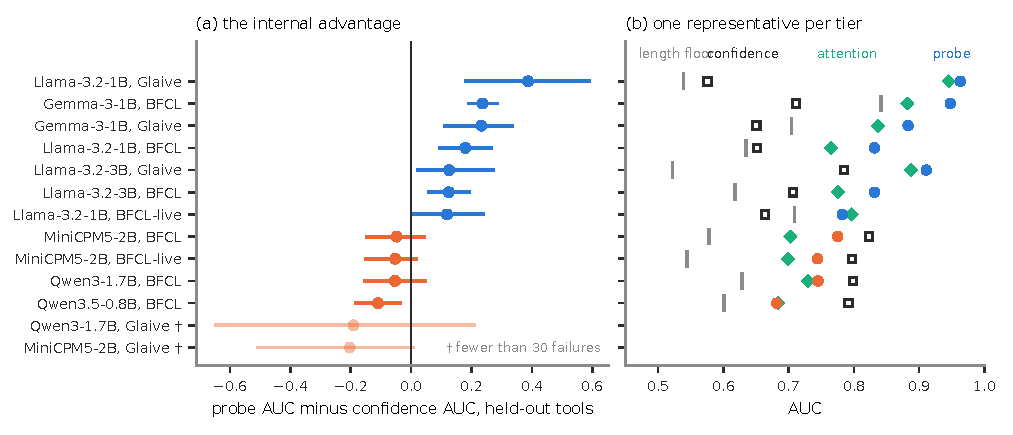
\includegraphics{fig1_gap}
\caption{(a) Token-role probe AUC minus mean log-probability AUC per run on held-out tools, dot at the mean over five split seeds, bar the 95\% interval from resampling tools. Blue Llama-3.2 and Gemma-3, orange Qwen3, Qwen3.5 and MiniCPM5, grey runs with fewer than thirty failures ($\dagger$). (b) Per run, the length floor, the mean log-probability, the better of the per-head profile and LapEigvals, and the probe, with the interval between log-probability and probe shaded.}
\label{fig:gap}
\end{figure*}


A language model agent acts by calling tools. When it calls the wrong one, or the right one with the wrong arguments, the call is usually well formed, so the runtime executes it and something happens in the world before anyone reads the transcript. A guardrail therefore has to judge the call in the interval between its generation and its execution, from what the model exposes in that single forward pass. Two kinds of evidence are available in that interval. The model's output distribution gives the probability it assigned to each token of the call, which every serving stack returns. The model's hidden states give a probe something to read, which only a stack that runs the model's own code can expose.

Detectors of the second kind work. A probe on the residual stream at the structural positions of a call, its function name, its argument values and its closing delimiter, separates wrong calls from right ones with high accuracy \citep{healy2026internal}, and linear probes on hidden states do so across many models \citep{yeats2026calls}. Diagnostics of the attention graph reach similar accuracy on related tasks \citep{binkowski2025lapeigvals,chuang2024lookback}. What none of these studies measures is the alternative the operator already has. The question this paper answers is whether reading the model's internals catches wrong tool calls that the model's own output confidence misses, and on which models.

We answer it with one quantity, the \emph{internal advantage}: the area under the curve of the residual-stream probe minus that of the mean token log-probability of the call, both scored on tools that never appeared in training and both reported beside a floor that reads only the length of the call. The comparison is run on small open-weight checkpoints from five model families, on three tool-calling benchmarks, under a protocol whose labelling and extraction code was audited and repaired before any number in this paper was computed, because the first version of that code scored correct list-valued calls as wrong on exactly the models where confidence then appeared useless.

The result can be stated in one sentence: on some models the output confidence already knows when a tool call is wrong, and on others only the hidden states do. On Llama-3.2 and Gemma-3 the probe leads confidence on every run, by a margin whose interval excludes zero in six runs of seven. On Qwen3, Qwen3.5 and MiniCPM5 the probe's lead is within noise of zero on every run and below zero with an interval excluding it on one. The two groups do not overlap at the level of the checkpoint, of which there are three on each side, too few for a test and enough for a description. The split does not follow model size (one and three billion parameters on the first side, 0.8 to two on the second), nor the format the model writes its calls in, nor release date alone, and it survives every alternative explanation we could test on the stored data: the difficulty of the items each model fails on, the number of labelled failures a probe is trained on, the choice of confidence summary, the benchmark, and the training population of the probe.

\paragraph{Contributions.}
\begin{enumerate}[topsep=1pt,itemsep=1pt,leftmargin=1.3em]
\item A controlled measurement of the internal advantage on \nRunsPowered{} powered runs from \nCkpt{} checkpoints in five families, with tools held out at test, a length floor in every table and a paired interval on every difference (\cref{sec:result}). \citet{healy2026internal} and \citet{yeats2026calls} establish that probes work. Neither scores the model's own confidence beside them, and \citet{yeats2026calls} splits by item rather than by tool.
\item The finding that whether a probe adds anything is a property of the model rather than of its size, with the controls that rule out item difficulty, label budget, the confidence summary, the benchmark and the probe's training population as explanations (\cref{sec:controls}).
\item A measurement of what the attention tier recovers where internals are needed: readouts that keep attention heads apart come within a few points of the probe, while head-averaged readouts sit near the length floor, with the controls that attribute the gap to head identity (\cref{sec:attention}).
\item The audit of the measurement chain itself, which found a labelling defect that had manufactured a family effect, with the record of the registered predictions, including one that failed and three not yet run (\cref{app:audit,app:registry}).
\end{enumerate}

\section{Related work}
\label{sec:related}

\paragraph{Probes on hidden states.}
Supervised probes on the residual stream recover whether a statement is true \citep{azaria2023internal,marks2024geometry}, predict hallucination risk from the query alone \citep{ji2024internal} and stand in for sampling-based uncertainty at the cost of one pass \citep{kossen2024sep}. \citet{orgad2025know} locate the signal at the exact-answer tokens, which is the observation the token-role probe of \citet{healy2026internal} applies to a call's name, arguments and delimiter. \citet{yeats2026calls} train linear probes on eighteen models on the same benchmark we use and find that model size and tool-specific fine-tuning predict probe accuracy. These results establish that the probe works. None of them scores the model's own output confidence on the same items, and none holds out the tool at test, which \cref{sec:setup} shows is where a tool-calling benchmark leaks.

\paragraph{Readouts of attention.}
Attention is the tensor a serving stack is most likely to expose without activations. LapEigvals trains a probe on the top eigenvalues of the attention Laplacian \citep{binkowski2025lapeigvals}, Lookback Lens on the share of attention paid to the context \citep{chuang2024lookback}, LLM-Check on eigenvalues of attention kernels \citep{sriramanan2024llmcheck}, SinkProbe on attention sinks \citep{binkowski2026sinks}, and graph-signal diagnostics on the Laplacian of a head-averaged attention graph \citep{noel2025gsp}. \citet{dahlem2026transport} prove that every transpose-invariant spectral diagnostic is blind to the direction of attention flow, and concurrent anonymous work proves that relabeling-invariant summaries, per-head Laplacian spectra included, cannot represent which token attends to which. We port the first four from their released code and treat them as the attention tier, with the same floor and the same held-out tools as the probe.

\paragraph{Output confidence.}
Language models' token probabilities are informative about their own correctness on question answering \citep{kadavath2022know}, and sampling-based estimates sharpen them \citep{farquhar2024semantic,manakul2023selfcheckgpt} at a cost in forward passes that an agent about to act does not have. Tool-calling benchmarks measure whether a call is right \citep{patil2025bfcl,patil2024gorilla,qin2024toolllm} and not whether the model's confidence tracks it. The contribution here is to put the single-pass confidence of the model beside the single-pass judges trained on its internals, under one protocol, and to find that which of them is needed depends on the model.

\section{Setup}
\label{sec:setup}

\paragraph{Task and labels.}
A model receives a user request and a set of tool schemas through its own chat template and generates greedily. The generated span is parsed for a tool call in whichever format the model writes, a JSON object for Llama-3.2, Gemma-3 and Qwen3 (the last inside call tags), and two XML dialects for Qwen3.5 and MiniCPM5, and compared with the benchmark's ground truth after both are normalised to a name and an argument dictionary. Each call receives a failure mode: valid, wrong name, wrong argument values, missing arguments, missing parallel calls, no call, an unparseable call, or a call cut off by the generation budget. On the benchmark category where no tool applies, the modes are a correct abstention or an over-triggered call. The binary label is valid against the rest. Every number is computed on the \emph{scored population}: items where a call is required and the generation is well formed enough to be judged, so a detector must separate a correct call from a wrong one rather than from prose or from a truncation. On Glaive, which has no abstention category, that is every well-formed call.

The labelling code was audited before the measurements in this paper, and its repairs are conditioning facts for every later number (\cref{app:audit}). The largest one concerns list-valued arguments: the ground truth of BFCL encodes each argument as a list of acceptable values, and the same unwrapping had been applied to the model's prediction, so a correct call carrying a list argument was scored as a wrong value. The defect fell on the JSON formats only. On the scored population it had turned \repPosBeforeQwenThreeBfcl{} labelled failures on Qwen3-1.7B into \repPosAfterQwenThreeBfcl{} (\repListFlipsQwenThreeBfcl{} correct calls with a list argument). A second repair, to the parsing of parallel calls that Llama-3.2 separates with semicolons, returned \repParallelLlamaThreeBBfcl{} calls of Llama-3.2-3B to the scored population and moved its failures from \repPosBeforeLlamaThreeBBfcl{} to \repPosAfterLlamaThreeBBfcl{}. Neither changed more than \labelChangedRecentMax{} labels on any run of the XML families. Two further repairs concern extraction: the probe positions were never located in the MiniCPM5 dialect, so its probe had read the end-of-sequence state three times, and Qwen3.5 generated past its end-of-turn token because that token was not among the stopping ids. Both runs were re-extracted, as were Gemma-3 on BFCL and one Llama-3.2-1B run. The remaining Llama-3.2 and Gemma-3 runs were relabelled under the corrected code but keep their original extraction, which carries a second beginning-of-sequence token, and \cref{tab:main} marks which is which. Two further Qwen3.5 checkpoints exist in the stored data, a 2B run with twenty-one failures, too few to score, and a 4B run extracted before the stopping repair whose stale internal advantage is $-0.07$. the 4B run is left out until it is re-extracted.

\paragraph{Models and benchmarks.}
\cref{tab:models} lists the checkpoints: Llama-3.2 at 1B and 3B, Gemma-3-1B, Qwen3-1.7B, Qwen3.5-0.8B and MiniCPM5-2B, released between 2024 and 2026, with dense, sliding-window and hybrid linear-attention stacks among them. The benchmarks are the Glaive function-calling corpus \citep{glaive2024}, the single-turn categories of BFCL-v4 including the category where no tool applies \citep{patil2025bfcl}, and the live categories of the same benchmark, contributed by its users rather than written for it. A run is one checkpoint on one benchmark. A run with fewer than thirty labelled items of either class on the scored population is marked underpowered, reported in every table and excluded from every aggregate.

\begin{table}[t]
\centering
\small
\caption{The model set. \emph{Reasoning mode} records whether the chat template carries a thinking mode, which is disabled at generation throughout. The column is discussed in \cref{sec:discussion}.}
\label{tab:models}
\begin{tabular}{@{}lllr@{}}
\toprule
Checkpoint & Released & Thinking mode & Runs \\
\midrule
Llama-3.2-1B & 2024-09 & no & 3 \\
Llama-3.2-3B & 2024-09 & no & 2 \\
Gemma-3-1B & 2025-03 & no & 2 \\
Qwen3-1.7B & 2025-04 & yes & 2 \\
MiniCPM5-2B & 2026-09 & yes & 3 \\
Qwen3.5-0.8B & 2026-02 & yes & 1 \\
\bottomrule
\end{tabular}

\end{table}

\paragraph{Detectors by access tier.}
\emph{Logits.} The mean token log-probability of the generated span, with its direction fixed on training items, is the confidence representative, chosen before any result was seen. Up to ten further length-invariant summaries (minimum, mean of the five least likely tokens, perplexity, fraction of tokens below one half, mean, maximum and final entropy, and three of these over the call's own tokens) are stored on the re-extracted runs and used in \cref{sec:controls}. \emph{Attention.} The per-head spectral profile, five eigenvalue-only metrics of the symmetric normalised Laplacian of each head's attention subgraph on the generated call. LapEigvals, SinkProbe and Lookback Lens from their authors' code. A head-averaged spectral profile as the literature's usual read. And an anchored readout of the call's own attention rows. \emph{Residual.} The token-role probe of \citet{healy2026internal}, a regularised logistic regression on the residual state at the function name, the mean over argument values and the closing delimiter at eight depths. And a token-level probe pooled over the span after \citet{obeso2025realtime}. \emph{Floor.} A classifier on prompt length, generation length and the truncation flag, which carries no information about the model's state.

\paragraph{Protocol.}
Items are grouped by ground-truth tool and split five ways at the group level, so every score is on tools absent from training. With item-level splits a classifier on the tool identity alone reaches high accuracy, because failures concentrate on particular tools. Every trained detector is fitted on the training folds restricted to the scored population, with a validation carve-out from training tools for its regularisation, and the direction of every untrained score is fixed on the same population. Each item is scored once, out of fold, and one pooled area under the curve is computed per split seed over five seeds. Every difference between two detectors is a paired bootstrap that resamples whole tools, with the percentile interval reported. The exact floor of any rank test over checkpoints is stated beside it.

\paragraph{The quantity.}
The internal advantage of a run is the pooled area under the curve of the token-role probe minus that of the mean log-probability, with its tool-resampled interval. A positive value means the probe catches wrong calls that confidence ranks as ordinary. We call the side of the split on which it is positive \emph{internals needed} and the other \emph{confidence suffices}, and both names are shorthand for the measured sign.

\section{The internal advantage depends on the model}
\label{sec:result}


\begin{table*}[t]
\centering
\small
\caption{Every run under the corrected labels and evaluator. $n_+$ and $n_-$ are the labelled failures and correct calls in the scored population, \emph{attention} the better of the per-head profile and LapEigvals, and the last column the internal advantage with its 95\% tool-resampled interval. $^{*}$ re-extracted under the corrected extractor. Other rows relabelled on their original extraction. $^\dagger$ fewer than thirty items of one class.}
\label{tab:main}
\begin{tabular}{llrrccccc}
\toprule
Model & Data & $n_+$ & $n_-$ & probe & attention & confidence & floor & probe $-$ confidence \\
\midrule
Llama-3.2-1B & Glaive & 223 & 357 & 0.957 & 0.947 & 0.579 & 0.540 & $+0.379$ [+0.15, +0.59] \\
Llama-3.2-1B & BFCL & 193 & 307 & 0.861 & 0.815 & 0.661 & 0.652 & $+0.200$ [+0.12, +0.27] \\
Llama-3.2-1B & BFCL-live & 209 & 156 & 0.780 & 0.795 & 0.661 & 0.707 & $+0.119$ [-0.00, +0.24] \\
Llama-3.2-3B & Glaive & 97 & 548 & 0.936 & 0.885 & 0.773 & 0.529 & $+0.163$ [+0.05, +0.29] \\
Llama-3.2-3B & BFCL & 157 & 539 & 0.884 & 0.833 & 0.712 & 0.621 & $+0.172$ [+0.11, +0.23] \\
Gemma-3-1B & Glaive & 158 & 460 & 0.883 & 0.837 & 0.650 & 0.704 & $+0.233$ [+0.11, +0.34] \\
Gemma-3-1B & BFCL & 379 & 135 & 0.949 & 0.903 & 0.707 & 0.866 & $+0.242$ [+0.19, +0.30] \\
\midrule
Qwen3-1.7B & BFCL & 64 & 627 & 0.791 & 0.745 & 0.741 & 0.616 & $+0.051$ [-0.06, +0.15] \\
Qwen3-1.7B$^\dagger$ & Glaive & 10 & 699 & 0.676 & 0.781 & 0.867 & 0.677 & $-0.191$ [-0.65, +0.21] \\
MiniCPM5-2B & BFCL & 67 & 627 & 0.808 & 0.758 & 0.815 & 0.564 & $-0.008$ [-0.13, +0.09] \\
MiniCPM5-2B & BFCL-live & 123 & 472 & 0.747 & 0.688 & 0.798 & 0.543 & $-0.051$ [-0.16, +0.02] \\
MiniCPM5-2B$^\dagger$ & Glaive & 9 & 716 & 0.710 & 0.713 & 0.913 & 0.685 & $-0.203$ [-0.51, +0.01] \\
Qwen3.5-0.8B & BFCL & 91 & 393 & 0.691 & 0.649 & 0.789 & 0.592 & $-0.099$ [-0.18, -0.02] \\
\bottomrule
\end{tabular}

\end{table*}

\cref{tab:main} and \cref{fig:gap} hold the paper's measurement. The \nRunsPowered{} powered runs fall into two groups that do not overlap. On the seven runs of Llama-3.2 and Gemma-3 the internal advantage runs from \gapInternalsMin{} to \gapInternalsMax{}, and its interval excludes zero on \nInternalsCiExcludesZero{} of them, the exception being Llama-3.2-1B on the live categories, where it touches zero. On the four powered runs of Qwen3, MiniCPM5 and Qwen3.5 it runs from \gapConfidenceMin{} to \gapConfidenceMax{}, its interval is above zero on none and below zero on \nConfidenceCiBelowZero{}. The same ordering holds for a probe that needs no call positions at all, the token-level probe pooled over the span: its advantage is \tokGapMinInternals{} to \tokGapMaxInternals{} on the first group and \tokGapMinConfidence{} to \tokGapMaxConfidence{} on the second. In practice, an operator of a Llama-3.2 or Gemma-3 agent who reads only the model's confidence passes most of the wrong calls that a probe would have stopped, and an operator of a Qwen3, Qwen3.5 or MiniCPM5 agent who builds a probe gains at most a few points over the confidence the model already reports.

Runs that share a checkpoint are not independent, so the unit for any test is the checkpoint, of which there are \nCkptInternals{} on each side. Their mean advantages separate completely, Llama-3.2-1B at \ckptGapLlamaOneB{}, Llama-3.2-3B at \ckptGapLlamaThreeB{}, Gemma-3-1B at \ckptGapGemma{} against Qwen3-1.7B at \ckptGapQwenThree{}, MiniCPM5-2B at \ckptGapMiniCpm{} and Qwen3.5-0.8B at \ckptGapQwenThreeFive{}. Three against three is the smallest attainable two-sided rank-test value, $p=\ckptExactFloor{}$, so the separation is reported as a description of these six checkpoints and not as a test, and \cref{sec:discussion} says what would test it.

Three properties of the model set do not separate the sides on their own. Size: the first side holds checkpoints of one and three billion parameters and the second of 0.8, 1.7 and two billion, and within Llama-3.2 the probe improves from 1B to 3B, as \citet{yeats2026calls} report across sizes, without the advantage changing sign. Call format: Qwen3 writes JSON like Llama-3.2 and Gemma-3 and sits on the other side. Attention design: MiniCPM5 is a dense stack like Llama-3.2, and Gemma-3 attends locally in all but four layers yet behaves like Llama-3.2. Release date comes closest, with every first-side checkpoint released by March 2025 and every second-side one from April 2025 on, and \cref{sec:discussion} returns to what that could mean.

\paragraph{Replication.} Llama-3.2-1B on BFCL was extracted twice, once before and once after the extraction repairs of \cref{sec:setup}, so the two runs differ in their generations as well as in their features. The internal advantage reads \replGapStale{} on the earlier extraction and \replGapClean{} on the later one, a drift of \replGapDelta{} that is inside the interval of either. Differences between detectors smaller than that drift are reported in the tables but not interpreted.

\section{What does not explain the split}
\label{sec:controls}

\begin{figure*}[t]
\centering
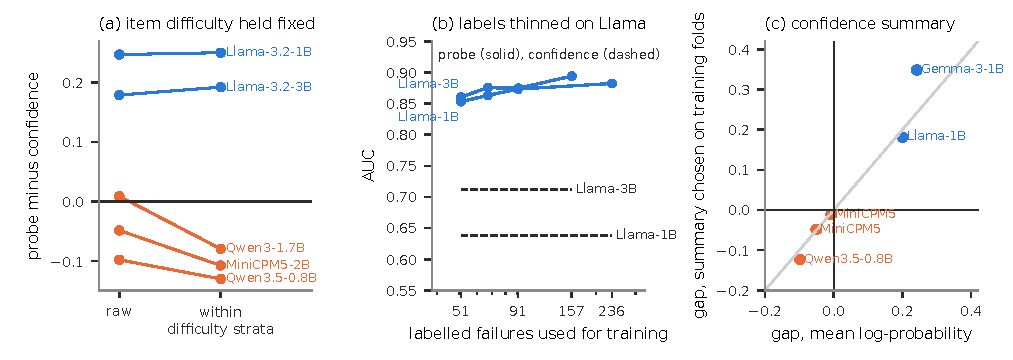
\includegraphics[width=\textwidth]{fig2_controls}
\caption{Three alternative explanations, each held fixed. (a) The internal advantage on the BFCL checkpoints, raw and recomputed within strata of item difficulty, where difficulty is the share of the other checkpoints that fail the same item. (b) The token-role probe's AUC on the two Llama-3.2 runs as its training failures are thinned to the counts the other families supply, with the mean log-probability dashed. (c) The advantage against the mean log-probability and against the confidence summary chosen on training folds, one point per run with stored summaries.}
\label{fig:controls}
\end{figure*}

A difference between model families is the kind of result that is usually something else, so each explanation that could produce it from the stored data was tested before it was believed. One of them, label error, did produce part of it and is reported first.

\paragraph{Labels and extraction.}
Before the audit of \cref{sec:setup}, Qwen3-1.7B appeared on the side where internals are needed, with an advantage of \gapQwenThreeBeforeAudit{}. Of its \repPosBeforeQwenThreeBfcl{} labelled failures on the scored population, \repPosAfterQwenThreeBfcl{} survive the repair of the list-argument comparison, and its advantage falls to \GapQwenThreeBfcl{}. The defect could not have produced the other side: it changed at most \labelChangedRecentMax{} labels on any Qwen3.5 or MiniCPM5 run, and the probe on MiniCPM5, which had read the end-of-sequence state for all three roles, moves by two points once it reads the call. On the re-extracted runs the probe's positions are located on \locatedMin{}\% or more of scored items, and the token-level probe, which needs none, orders the sides the same way (\cref{sec:result}). A reviewer should read the earlier family effect as an artefact and the present one as what survives its removal.

\paragraph{Item difficulty.}
A model that fails rarely fails on hard items, and its confidence may register that an item is hard rather than that its own call is wrong. The items of BFCL are the same text for every model, so an item's difficulty is the share of the other checkpoints that fail it, and that share alone predicts a model's failures at \diffOnlyMin{} to \diffOnlyMax{} AUC. Recomputing the probe and the confidence inside strata of that difficulty, weighted by the positive-negative pairs each stratum holds, removes everything either detector gains from knowing which items are hard. The split widens (\cref{fig:controls}a): the advantage moves from \diffGapRawLlamaOneB{} to \diffGapWithinLlamaOneB{} on Llama-3.2-1B and from \diffGapRawMiniCpm{} to \diffGapWithinMiniCpm{} on MiniCPM5-2B. Confidence on the models where it suffices is tracking the model's own errors, not the hardness of the request.

\paragraph{Label budget.}
A probe needs labelled failures and confidence needs none, and the models where confidence suffices fail less often, supplying \nPosQwenThreeBfcl{} to \nPosQwenThreeFiveBfcl{} failures against hundreds on Llama. Training the Llama probes on exactly those counts, with the test folds untouched, costs them \budgetProbeDropLlamaOneB{} AUC at 1B and \budgetProbeDropLlamaThreeB{} at 3B (\cref{fig:controls}b). At \budgetMinPosLlamaOneB{} training failures the advantage is still \budgetGapAtMinLlamaOneB{} and \budgetGapAtMinLlamaThreeB{}, both above every value on the other side at any budget.

\paragraph{The confidence summary.}
The mean log-probability is one summary of the output distribution. On the runs that store eleven length-invariant summaries, the one with the highest AUC on the other folds' items is applied fold by fold, so no summary is chosen on the items it is scored on (\cref{fig:controls}c). Two runs on the side where internals are needed store several summaries: on Llama-3.2-1B on BFCL the fold-chosen summary moves the advantage from \GapLlamaOneBBfcl{} to \gapBestLlamaOneBBfcl{}, and on Gemma-3-1B on BFCL the fold-chosen summary generalises worse than the mean and the advantage rises to \gapBestGemmaBfcl{}. On the other side the largest value is \gapBestConfidenceMax{}. An oracle that picks the best single summary on the test items, which no deployment could do, leaves the first side at \gapOracleMinInternals{} to \gapOracleMaxInternals{} and the second at \gapOracleMinConfidence{} to \gapOracleMaxConfidence{}. Two summaries that grow with the length of the call, its token count and its total log-probability, are excluded from the candidates because they are length features, which the floor already covers.

\paragraph{Benchmark.}
Gemma-3 reads \GapGemmaGlaive{} on Glaive and \GapGemmaBfcl{} on BFCL, Llama-3.2-1B reads \GapLlamaOneBGlaive{}, \GapLlamaOneBBfcl{} and \GapLlamaOneBLive{} across three benchmarks, and MiniCPM5 reads \GapMiniCpmBfcl{} and \GapMiniCpmLive{} on two, so no run's side depends on its benchmark. Qwen3 and MiniCPM5 on Glaive are underpowered, with \nPosQwenThreeGlaive{} and \nPosMiniCpmGlaive{} failures in several hundred calls, and their intervals span zero. That they almost never fail there is itself consistent with their side.

\paragraph{Training population and pooling.}
Two protocol choices move the numbers and are fixed as stated in \cref{sec:setup}. Training the probe on every item while scoring the call-required population teaches it the format failures that population excludes, and on BFCL the same behaviour, answering without a call, is a failure on one category and a success on another. Training on the scored population removes a spurious family difference on the population that includes abstentions and changes the call-required numbers by less than the replication drift. Fixing the sign of the log-probability on the scored population rather than on every item raises confidence on two Llama runs by up to a quarter of the AUC scale without moving their side. Pooling out-of-fold scores across folds with different calibrations penalises a fitted probe and not a fixed confidence score: the advantage computed within folds is higher than the pooled one by \poolShiftMean{} on average and \poolShiftMax{} at most, and ranges from \gapWithinMinInternals{} to \gapWithinMaxInternals{} on the first side and \gapWithinMinConfidence{} to \gapWithinMaxConfidence{} on the second.

\paragraph{A registered prediction that failed.}
Before the audit, the split had been written down as a division by release period, the two 2026 families against the three earlier ones, with a decision rule committed to the repository. That prediction failed: Qwen3, released in April 2025, sits with the 2026 families once the labels are right. A cutoff placed one month later would have passed, which is why the division that holds is reported as a description and the property behind it as a hypothesis (\cref{app:registry}).

\section{Reading attention where internals are needed}
\label{sec:attention}

\begin{figure}[t]
\centering
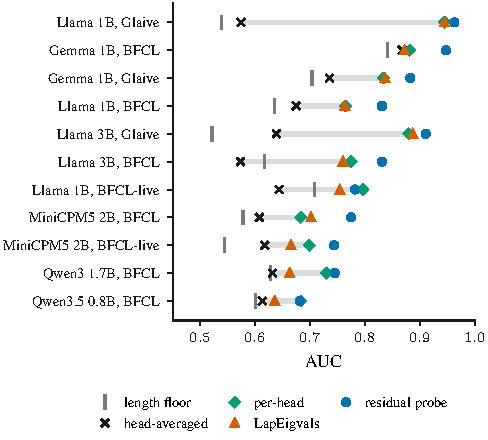
\includegraphics[width=\columnwidth]{fig3_attention}
\caption{The attention tier on every powered run: the length floor, the head-averaged spectral profile, the per-head profile, LapEigvals and the token-role probe. Keeping heads apart moves the attention readout from the floor to within a few points of the probe.}
\label{fig:attention}
\end{figure}

An operator whose stack exposes attention weights but not activations wants to know how much of the probe an attention-only readout recovers. On the runs where internals are needed, the per-head spectral profile and LapEigvals trail the token-role probe by a few points (\cref{fig:attention}): \GapProbePerHeadLlamaOneBBfcl{} on Llama-3.2-1B and \GapProbePerHeadGemmaBfcl{} on Gemma-3-1B on BFCL, with the two attention readouts within noise of each other on every run (per-head minus LapEigvals \GapPerHeadLapEigLlamaOneBBfcl{} and \GapPerHeadLapEigGemmaBfcl{}). SinkProbe and the anchored readout of the call's own rows sit in the same band. On the runs where confidence suffices every attention readout sits below confidence, as the probe does.

What decides whether an attention readout works at all is whether the heads are averaged before anything is computed. The head-averaged spectral profile, which is how most of this literature reads a layer, does not clear the length floor on several runs, and keeping heads apart is worth \GapPerHeadAvgLlamaOneBBfcl{} on Llama-3.2-1B on BFCL. On the stored per-head features of \ladNRuns{} runs, averaging the five metrics over heads after computing them per head scores \ladMetricAvg{}, keeping them apart \ladPerHead{}, a gain of \ladGainPerHead{} that is positive on \ladGainPerHeadPos{} of \ladNRuns{} runs; permuting the head axis independently for every item, which keeps every value and destroys only which head produced it, costs \ladGainVsShuffle{}, and padding the averaged features with noise to the per-head width changes them by \ladNoiseEffect{}. The signal is in which head does what.

The reason is elementary and we state it once. Any functional of the head-averaged attention graph is constant on head configurations that share a mean, so no averaged read can represent the contrast between heads (\cref{prop:annihilation}). For the algebraic connectivity in particular, the averaged graph can only overstate it, since the second Laplacian eigenvalue is a pointwise minimum of linear functionals and hence concave, with equality exactly when every head shares a Fiedler vector (\cref{prop:jensen}); on the layers we measured the averaged graph reports connectivity well above the mean over heads throughout. LapEigvals already keeps heads apart, and its authors note that the causal Laplacian is triangular so its eigenvalues are its diagonal \citep{binkowski2025lapeigvals}; those features are therefore an in-degree sequence, invariant to any rewiring that preserves degrees, while a symmetrised spectrum is a global functional of the routing, which is why two such different readouts perform alike once heads are kept apart (\cref{app:proofs}). Concurrent anonymous work proves that neither can represent which token attends to which, and that a readout anchored on a distinguished row can; on tool calls the anchored readout ties the per-head profile (\GapAnchPerHeadLlamaOneBBfcl{} and \GapAnchPerHeadGemmaBfcl{}), so the limit it identifies is not what separates attention from the residual stream here.

\section{Deployment}
\label{sec:deployment}

\begin{figure}[t]
\centering
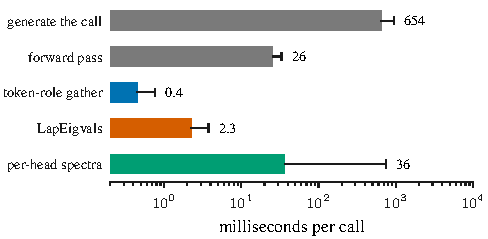
\includegraphics[width=\columnwidth]{fig4_cost}
\caption{Cost per call of each path on Llama-3.2-1B, median over \latNPrompts{} BFCL prompts on one consumer GPU, with a line to the 90th percentile. Every internal judge needs the forward pass. The per-head spectra add eigendecompositions on the call span.}
\label{fig:cost}
\end{figure}

\paragraph{Cost.}
Reading confidence costs nothing beyond generation. Every internal judge needs one teacher-forced pass over prompt and call, \latPass{}\,ms against \latGen{}\,ms of generation on the hardware of \cref{fig:cost}. A stack that keeps the generation pass's states can skip it for the residual tier but not for attention, whose probabilities a fused kernel never materialises. On top of that pass the token-role features cost \latTokenRole{}\,ms and LapEigvals \latLapEig{}\,ms. The per-head spectra cost \latPerHead{}\,ms at the median, \latPerHeadPct{}\% of generation, and \latPerHeadNinety{}\,ms at the 90th percentile, more than generation itself when the call is long.

\paragraph{Calls with a history.}
An agent's calls are made with a conversation behind them. On the multi-turn categories of BFCL-v4, replayed with the ground-truth calls of the two preceding turns in the prompt, and in half the records with one of those turns replaced by a wrong call reported as successful, MiniCPM5-2B's failure rate moves from \mtFailClean{}\% after a clean history to \mtFailCorrupt{}\% after a corrupted one (Fisher $p=\mtFisherP{}$). The probe reads \mtAucProbe{} against \mtAucConf{} for confidence, and a probe trained on clean histories only scores corrupted items at \mtAucProbeCleanOnCorrupt{} against \mtAucProbeCleanOnClean{} on clean ones. On this one model, the side of the split and the usefulness of a judge trained without failed trajectories both carry over to a call made with a history (\cref{app:multiturn}).

\begin{tcolorbox}[colback=white,colframe=black!60,boxrule=0.5pt,arc=1pt,left=4pt,right=4pt,top=3pt,bottom=3pt,title=\small Before building an internal judge for a tool-calling model]
\small
\begin{enumerate}[topsep=0pt,itemsep=1pt,leftmargin=1.2em]
\item Score the mean token log-probability on a few hundred labelled calls from the model to be deployed, on tools absent from the labelled set. If it already separates wrong calls well, no probe we trained improved on it (\cref{tab:main}, lower block). Cost of skipping: a probe, its labels and a forward pass per call for a gain of at most \gapConfidenceMax{} AUC.
\item If it does not, train the token-role probe on the residual stream. Fifty labelled failures suffice (\cref{fig:controls}b). Cost of skipping: \gapInternalsMin{} to \gapInternalsMax{} AUC against confidence.
\item Where only attention is exposed, read it per head. Cost of averaging heads first: \phHavgMinInternals{} to \phHavgMaxInternals{} AUC where internals are needed.
\item Split the labelled set by tool and keep a length floor beside every number. Cost of skipping: a classifier on the tool identity alone looks like a detector.
\end{enumerate}
\end{tcolorbox}

\section{Discussion}
\label{sec:discussion}

\paragraph{What the split could be.}
With five families the data say which models fall on which side and not why, and \cref{tab:models} offers two readings that both fit all six checkpoints. One is release date, with a cutoff between March and April 2025. The other, recorded as a hypothesis before any new model was extracted (\cref{app:registry}), is the post-training recipe: the three families on which confidence suffices all ship a chat template with a reasoning mode and were post-trained with it, and the two on which internals are needed do not. Post-training that rewards a model for working through a call before writing it may also leave its token probabilities tracking its own errors. \citet{yeats2026calls} find that tool-specific fine-tuning lowers what a probe reads by about five points, which is consistent with a model whose post-training moves information about its own errors toward its output. The two readings are separated by matched pairs that differ in post-training on one base model, Qwen3 generated with its reasoning mode on against off, or an instruction-tuned base against its reasoning-tuned sibling, and the first of these runs on the hardware of this study. A third reading, that a model which has seen the benchmark in training fails less and knows when it fails, is weakened by the live categories, contributed by users after the curated set, on which MiniCPM5 behaves as it does on the curated one, but it is not excluded.

\paragraph{For operators.}
The decision that changes is whether to build an internal judge at all. If the deployed model's log-probability already ranks its wrong calls, as it does on Qwen3, Qwen3.5 and MiniCPM5 here, the probe adds at most \gapConfidenceMax{} AUC and costs a forward pass per call. If it does not, as on Llama-3.2 and Gemma-3, the probe adds \gapInternalsMin{} to \gapInternalsMax{} and fifty labelled failures are enough to fit it. Both are answered by scoring confidence on a few hundred labelled calls from that model, which is cheaper than either mistake.

\paragraph{For model builders.}
A model whose confidence tracks its tool-calling errors ships its own guardrail. If the post-training reading above holds, that property is a choice made in training and can be measured as part of a release, by the same protocol: the internal advantage on held-out tools against a length floor.

\paragraph{For detector research.}
Reporting a probe's accuracy without the model's own confidence beside it, on items rather than tools, can show a strong detector on a model that did not need one. The two findings that survive every control here, that the need for a judge is a property of the model and that attention must be read per head where a judge is needed, both appear only under that comparison.

\section{Limitations}
\label{sec:limitations}

The first limitation is the instrument. Labels come from comparing a call with a benchmark's ground truth, which is a proxy for whether the action would have been harmful, and the audit of \cref{app:audit} shows that a parser can manufacture a family effect. A hand-checked sample of twenty-five items per run put the label error between zero and one in five on the JSON dialects before the repair and near zero on the XML dialects, and \cref{app:audit} reports the error measured on the repaired labels; what residual error remains inflates probes, because a mislabelled correct call has a surface form a probe can learn and confidence cannot, so it would move the result toward the side where internals appear needed.

The second is scale and breadth. Every checkpoint is at most three billion parameters and every family is represented by one or two checkpoints, so the two sides hold three checkpoints each, which is below what any test can separate, and the property that divides them is a hypothesis. Agents in production run on models of eight billion parameters and above, and \citet{yeats2026calls} find probe accuracy rising with size; whether confidence rises with it is the open question the matched pairs of \cref{sec:discussion} would answer.

The third is realism. Calls are single-step on three benchmarks of English requests, and the multi-turn evaluation replays the benchmark's own earlier calls rather than the model's trajectory with executed tool results, so it shows that a judge is not disturbed by a wrong call in the history and cannot show what a wrong tool result does. Cost is measured on one consumer GPU and not on a serving stack.

The last is direction. The two protocol choices of \cref{sec:controls} that move the numbers, the training population and the sign-fixing population, both moved them toward confidence, and the confidence summary chosen on training folds moves the Llama advantage down by \bestConfShrinkMax{} at most; nothing we found moves the Qwen3, Qwen3.5 or MiniCPM5 advantage up. The result should therefore be read as a lower bound on how often confidence suffices and an upper bound on where internals are needed.


\section*{Impact statement}
This work measures open-weight language models on public tool-calling benchmarks, trains no model and involves no human subjects. Its aim is defensive: to tell an operator when a wrong tool call can be caught from the model's own state before it executes, and when the model's output confidence already does so. The same detectors could in principle guide the construction of calls that evade them, which is why we report operating points and the models on which each detector weakens rather than one headline number.

\section*{Reproducibility statement}
Every number in this paper expands from a macro that a released script builds from the result files, and each macro records the file, field and run it reads. Labels are recomputed from the stored generations at evaluation time, so the labelling rule in force is the one in the released code. Splits are grouped by ground-truth tool, every intervals resamples tools, and the registered predictions of \cref{app:registry} were committed before the data that test them. Models and benchmarks are public and the released repository regenerates every table and figure from the stored extractions.

\bibliography{references}
\bibliographystyle{icml2026}

\appendix
\onecolumn
\clearpage
\addtocontents{toc}{\protect\setcounter{tocdepth}{2}}
\makeatletter
\renewcommand*\l@section{\@dottedtocline{1}{0em}{2.0em}}
\renewcommand*\l@subsection{\@dottedtocline{2}{2.0em}{2.8em}}
\makeatother
\renewcommand{\contentsname}{Appendix contents}
{\small\setlength{\parskip}{0pt}\tableofcontents}
\medskip

\section{Proofs}
\label{app:proofs}

Fix one layer with $H$ heads and $T$ positions. Head $h$ produces a row-stochastic attention matrix $A_h$, symmetrised and stripped of self-loops into $W_h = \tfrac12(A_h + A_h^\top) - \operatorname{diag}(\tfrac12(A_h + A_h^\top))$, with combinatorial Laplacian $L_h = D_h - W_h$ and symmetric normalised Laplacian $\mathcal{L}_h = I - D_h^{-1/2} W_h D_h^{-1/2}$. The head-averaged graph is $\bar W = \frac1H \sum_h W_h$. $\lambda_2$ denotes the second-smallest eigenvalue.

\begin{proposition}[annihilation]
\label{prop:annihilation}
Any map of the form $\{W_h\} \mapsto \Phi(\bar W)$ is constant on every set of head configurations sharing the same mean, and for every $H \ge 2$ and $T \ge 3$ there exist admissible configurations with the same mean whose per-head connectivities differ by a constant independent of $T$.
\end{proposition}
\begin{proof}
The first claim holds because $\Phi$ factors through $\bar W$. For the second let $P$ be the path on $T$ nodes with weights $\tfrac12$ and $K$ the complete graph with weights $1/(T-1)$; both have row sums at most one and so arise from row-stochastic attention under the construction above, as does their mean. Put $W_1 = P$, $W_2 = K$ and $W_1' = W_2' = \tfrac12(P + K)$, repeating the pattern for $H > 2$. The two configurations share the mean $\tfrac12(P+K)$, while $\lambda_2(L_P) = 1 - \cos(\pi/T)$ and $\lambda_2(L_K) = T/(T-1) > 1$.
\end{proof}

\begin{proposition}[head averaging overstates connectivity]
\label{prop:jensen}
For any heads $W_1, \dots, W_H$, $\lambda_2(\bar L) \ge \frac1H \sum_h \lambda_2(L_h)$, with equality if and only if the heads admit a common Fiedler vector.
\end{proposition}
\begin{proof}
The Laplacian is linear in the adjacency, so $\bar L = \frac1H \sum_h L_h$. By Courant--Fischer, $\lambda_2(L) = \min_{x \perp \mathbf 1, \|x\|=1} x^\top L x$ is a pointwise minimum of linear functionals of $L$ and hence concave on the cone of graph Laplacians; Jensen's inequality gives the bound. If $x^\star$ attains the minimum for $\bar L$ then $\lambda_2(\bar L) = \frac1H \sum_h x^{\star\top} L_h x^\star \ge \frac1H \sum_h \lambda_2(L_h)$, with equality exactly when $x^\star$ is a Fiedler vector of every head \citep{chung1997spectral}.
\end{proof}

On \ensuremath{210} layers from three models and three inputs the combinatorial inequality holds with no violation and a gap bounded away from zero; for the normalised Laplacian the detectors use, where the Rayleigh quotient is not linear in $W$ and the inequality is not a theorem, it holds on all but three layers, and the averaged graph reports connectivity a median fourteen percent above the mean over heads. The mean pairwise alignment of per-head Fiedler vectors is \ensuremath{0.45}, far from the value one that equality needs.

\begin{remark}[LapEigvals reads degrees]
\label{rem:lapeig}
\citet{binkowski2025lapeigvals} observe that for a causal attention matrix the Laplacian $L = D - A$ is lower triangular, so its spectrum is its diagonal $\{d_j - A_{jj}\}$. Their top-$k$ features therefore depend on $A$ only through its column sums and diagonal, and two causal attention matrices with the same in-degree sequence and self-attention weights yield identical features however differently they route attention. The symmetrisation above destroys triangularity, so the spectra the per-head profile reads are global functionals of the routing. The two families are not two estimates of one object, and the fact that both keep heads apart is what they share.
\end{remark}

\section{Protocol details}
\label{app:protocol}

\paragraph{Generation.} Greedy decoding in bfloat16 with deterministic kernels, a budget of 256 new tokens (160 on multi-turn prompts), tool schemas passed through the model's chat template with its reasoning mode disabled, and every end-of-turn id of the template among the stopping ids. The rendered text is tokenised without a second beginning-of-sequence token. Each record stores its budget, library versions and commit.

\paragraph{Features.} Per-head spectra, LapEigvals, SinkProbe, Lookback and anchored features are reduced inside a forward hook on each attention module, so a layer's probabilities are released before the next layer computes; the eigendecompositions are taken on the subgraph induced on the generated call. Residual states are read at eight depths spaced by \texttt{linspace} over the layer count at the function-name token, the mean over argument-value tokens and the closing delimiter, located by alignment of the parsed call to the token offsets in each dialect; each record stores whether a call was located, and the probe is scored on every item regardless. Per-token states for the token-level probe cover 128 generated tokens.

\paragraph{Classifiers.} Logistic regression with $\ell_2$ penalty, standardised features, class balancing and $C \in \{0.01, 0.1, 1, 10\}$ chosen on the validation carve-out; LapEigvals and SinkProbe widths $k \in \{5, 10, 25, 50, 100\}$ chosen the same way; gradient-boosted trees with a logistic fallback for the head-averaged per-layer sets.

\paragraph{Scoring.} Five tool-grouped folds with a one-fifth validation carve-out of training tools, training restricted to the scored population, one pooled AUC per seed over five seeds, mean reported. Differences are paired bootstraps over items that resample whole tools, 2000 draws, percentile intervals, Holm-adjusted within each run's family of contrasts for the appendix table.

\section{Labelling and extraction defects found by the audit}
\label{app:audit}

Each defect was present in a working pipeline, produced a plausible number and was found by auditing the code rather than the results. The direction column says which side of the comparison it favoured.

\begin{center}\small
\begin{tabular}{p{0.38\linewidth}p{0.26\linewidth}p{0.28\linewidth}}
\toprule
Defect & Where it fell & Favoured \\
\midrule
A predicted list argument was collapsed to its first element by the unwrapping meant for ground truth, so correct list-valued calls were scored wrong & JSON dialects (Llama-3.2, Qwen3); \labelPosBeforeQwenThreeBfcl{}\,$\to$\,\labelPosAfterQwenThreeBfcl{} failures on Qwen3-1.7B & probes, through a surface feature \\
Semicolon-separated parallel calls did not parse and were scored unparseable & Llama-3.2-3B, \labelPosBeforeLlamaThreeBBfcl{}\,$\to$\,\labelPosAfterLlamaThreeBBfcl{} failures & probes \\
A list sent as a string was compared inconsistently with a list & Llama-3.2 & probes \\
A truncated call reached the scored population through modes other than unparseable & all, few items & neither \\
Probe positions never located in the MiniCPM5 dialect, so the probe read the end-of-sequence state for every role & MiniCPM5 & confidence, by \ensuremath{0.02} \\
Generation stopped only on end-of-text, so Qwen3.5 ran past its end of turn and every span feature carried extra tokens & Qwen3.5 & unclear, small \\
A second beginning-of-sequence token & Llama-3.2, MiniCPM5 & neither \\
Probes trained on every item and scored on a subset learned format failures the subset excludes & population including abstentions & probes on the models that make format failures \\
The sign of the log-probability fixed on items it is never scored on & Llama-3.2 on two runs & probes, by up to \ensuremath{0.24} \\
Runs sharing a checkpoint treated as independent in a rank test & aggregate & the apparent significance \\
\bottomrule
\end{tabular}
\end{center}

A hand-checked sample of twenty-five items per run before the repairs put the label error at zero to one in five on the JSON dialects and at most one in twenty-five on the XML dialects; the measured error on the repaired labels is reported in the released audit file.

\section{Registered predictions and outcomes}
\label{app:registry}

\begin{center}\small
\begin{tabular}{p{0.06\linewidth}p{0.42\linewidth}p{0.44\linewidth}}
\toprule
Id & Prediction, committed before the data that test it & Outcome \\
\midrule
R1 & The internal advantage separates the families by release period: MiniCPM5 and Qwen3.5 below Llama-3.2, Gemma-3 and Qwen3 at every checkpoint. & Failed. Qwen3-1.7B moved to the confidence side once the list-argument defect was repaired (\cref{tab:main}). The division that holds was found afterwards and is descriptive. \\
C1 & The per-head spectral score and LapEigvals are not interchangeable, each keeps signal when the other is conditioned on, and their union exceeds both. & Two held, the third failed (union gain within noise on eleven runs). \\
H1 & Models whose post-training included a reasoning mode have an internal advantage lower by at least 0.05 than a matched model without it, same base. & Registered; needs matched pairs above the size of this study. \\
H2 & Within one model the advantage is within 0.05 of its full value under a tenfold cut of labels and under added distractor tools. & The label half holds (\cref{fig:controls}b); the distractor half is not yet run. \\
\bottomrule
\end{tabular}
\end{center}

\section{Every detector on every run}
\label{app:detectors}

\begin{center}\scriptsize
\begin{tabular}{llcccccccccc}
\toprule
Model & Data & token-role & token-level & head-avg. & per-head & LapEigvals & Lookback & SinkProbe & anchored & log-prob & floor \\
\midrule
Llama-3.2-1B & Glaive & 0.957 & 0.971 & 0.602 & 0.947 & 0.936 & 0.940 & -- & -- & 0.579 & 0.540 \\
Llama-3.2-1B & BFCL & 0.861 & 0.832 & 0.675 & 0.812 & 0.815 & 0.792 & 0.833 & 0.806 & 0.661 & 0.652 \\
Llama-3.2-1B & BFCL-live & 0.780 & 0.774 & 0.643 & 0.795 & 0.752 & 0.804 & -- & -- & 0.661 & 0.707 \\
Llama-3.2-3B & Glaive & 0.936 & 0.863 & 0.607 & 0.885 & 0.864 & 0.883 & -- & -- & 0.773 & 0.529 \\
Llama-3.2-3B & BFCL & 0.884 & 0.846 & 0.629 & 0.833 & 0.822 & 0.832 & -- & -- & 0.712 & 0.621 \\
Gemma-3-1B & Glaive & 0.883 & 0.898 & 0.736 & 0.834 & 0.837 & 0.786 & -- & -- & 0.650 & 0.704 \\
Gemma-3-1B & BFCL & 0.949 & 0.946 & 0.884 & 0.903 & 0.898 & 0.928 & 0.929 & 0.935 & 0.707 & 0.866 \\
Qwen3-1.7B & BFCL & 0.791 & 0.734 & 0.642 & 0.745 & 0.727 & 0.778 & -- & -- & 0.741 & 0.616 \\
Qwen3-1.7B$^\dagger$ & Glaive & 0.676 & 0.790 & 0.445 & 0.781 & 0.678 & 0.709 & 0.702 & 0.674 & 0.867 & 0.677 \\
MiniCPM5-2B & BFCL & 0.808 & 0.810 & 0.670 & 0.736 & 0.758 & 0.780 & 0.799 & 0.789 & 0.815 & 0.564 \\
MiniCPM5-2B & BFCL-live & 0.747 & 0.737 & 0.622 & 0.688 & 0.673 & 0.721 & 0.705 & 0.699 & 0.798 & 0.543 \\
MiniCPM5-2B$^\dagger$ & Glaive & 0.710 & 0.760 & 0.635 & 0.713 & 0.652 & 0.723 & 0.690 & 0.773 & 0.913 & 0.685 \\
Qwen3.5-0.8B & BFCL & 0.691 & 0.719 & 0.617 & 0.649 & 0.609 & 0.664 & 0.660 & 0.728 & 0.789 & 0.592 \\
\bottomrule
\end{tabular}

\end{center}

\section{Confidence summaries}
\label{app:confidence}

On the re-extracted runs eleven length-invariant summaries of the token log-probabilities are stored per call: the mean, the minimum, the mean of the five least likely tokens, the perplexity, the fraction of tokens below one half, the mean, maximum and final predictive entropy, and the mean, minimum and mean-of-five over the call's own tokens with special tokens removed. For each cross-fit fold the summary with the highest AUC on the items of the other folds is applied to the fold's items; the pooled score is one detector chosen fold by fold on data it is not scored on. On Llama-3.2-1B on BFCL the chosen summary reaches \aucBestConfLlamaOneBBfcl{} against \aucConfLlamaOneBBfcl{} for the mean, and the advantage becomes \gapBestLlamaOneBBfcl{} [\gapBestLoLlamaOneBBfcl{}, \gapBestHiLlamaOneBBfcl{}]. On Qwen3.5-0.8B the chosen summary reaches \aucBestConfQwenThreeFiveBfcl{} and the advantage \gapBestQwenThreeFiveBfcl{} [\gapBestLoQwenThreeFiveBfcl{}, \gapBestHiQwenThreeFiveBfcl{}]. Two summaries that grow with the call's length, its token count and its total log-probability, are excluded; on Gemma-3-1B on BFCL the token count alone reaches \ensuremath{0.87}, which is the length floor of that run and not a confidence.

\section{Head resolution controls}
\label{app:ladder}

On the stored per-head features of \ladNRuns{} runs, under the same classifier and splits: the head-averaged graph's five metrics score \ladGraphAvg{}, the same five metrics computed per head and then averaged \ladMetricAvg{}, all heads kept \ladPerHead{}, the averaged features padded with Gaussian noise to the per-head width \ladNoisePadded{}, and the per-head features with the head axis permuted independently per item \ladHeadShuffled{}. The gain of keeping heads apart over averaging the metrics is \ladGainPerHead{} and positive on \ladGainPerHeadPos{} runs; destroying head identity costs \ladGainVsShuffle{}; width without information changes the averaged read by \ladNoiseEffect{}.

\section{Multi-turn protocol}
\label{app:multiturn}

The four multi-turn categories of BFCL-v4 (base, missing parameter, missing function, long context), one record per turn up to the fourth, with the ground-truth calls of the two preceding turns rendered as assistant messages each followed by a fixed acknowledgement. In the cascade condition one of the two preceding turns carries a call drawn from another conversation, with the same acknowledgement. Conversations with more than 22 tools are skipped. Folds group items that share either a tool or a conversation. Labels penalise arguments the schema does not define, because a weak model echoes tool schemas into argument-less calls on these prompts. On \mtN{} turns of MiniCPM5-2B the failure rate is \mtFailClean{}\% after a clean history and \mtFailCorrupt{}\% after a corrupted one.

\section{Models and versions}
\label{app:models}

\begin{center}\small
\begin{tabular}{llll}
\toprule
Checkpoint & Released & Attention & Layers read \\
\midrule
meta-llama/Llama-3.2-1B-Instruct & 2024-09 & dense GQA, 16 layers, 32 heads & all \\
meta-llama/Llama-3.2-3B-Instruct & 2024-09 & dense GQA, 28 layers, 24 heads & all \\
google/gemma-3-1b-it & 2025-03 & sliding window with 4 global layers, 4 heads & all \\
Qwen/Qwen3-1.7B & 2025-04 & dense GQA, 28 layers, 16 heads & all \\
Qwen/Qwen3.5-0.8B & 2026-02 & hybrid, softmax in 6 of 24 layers & softmax layers \\
openbmb/MiniCPM5-2B & 2026-09 & dense, 42 layers, 16 heads & all \\
\bottomrule
\end{tabular}
\end{center}

Experiments were run on a single 16\,GB consumer GPU. Library versions, the generation seed and the commit are recorded in every extraction.


\end{document}
